\documentclass[%
 superscriptaddress,
%  prl,
 aip,
 %jmp,%
 amsmath,amssymb,
preprint,%
% reprint,%
 author-year,%
%author-numerical,%
longbibliography
]{revtex4-2}

% Colin Ophus - 2021 April
% This is a template for M&M papers, based on revtex

% packages
\usepackage{
amsmath,
amssymb,
bm,  
color,
comment,
dcolumn,
enumerate,
float,
graphicx,
hyperref,
mathrsfs,
tabularx,
titlesec,
soul,
subfigure,
listings
}

\usepackage{appendix}

% set lsiting 
\definecolor{gray}{rgb}{0.75,0.75,0.75}
\lstset{numbers=left, 
                language=Python,
                basicstyle=\footnotesize,
                captionpos=b,
                %title=\lstname,
                %backgroundcolor=\color{gray},
                numberstyle=\footnotesize, 
                numbersep=10pt,
                basicstyle=\footnotesize,
                frame=shadowbox,
                breaklines=true,
                numbersep=5pt,
                xleftmargin=0.5in,
                xrightmargin=0.5in}
% Hyperlink and in-doc link setup

\definecolor{linkColor}{rgb}{0.7,0,0}
\definecolor{darkred}{rgb}{0.7,0,0}
\hypersetup{pdfborder={0 0 0},colorlinks=true,urlcolor=linkColor,citecolor=linkColor}

% Define various commands
\newcommand{\ii}{{i\mkern1mu}}
% \newcommand{\vect}[1]{\mathbf{#1}}
% \newcommand{\Smat}{\mathcal{S}}
% \newcommand{\ft}{\mathcal{F}}
% \newcommand{\ift}{\mathcal{F}^{-1}}
% \newcommand{\angstroms}{\text{\normalfont\AA}}
% \newcommand{\f}[2][]{\mathcal{F}_{#1}\left[#2\right]}
% \renewcommand{\vec}[1]{\mathbf{#1}}
% \newcommand{\mvec}[1]{\bm{#1}}
% \newcommand{\smatrix}[0]{$\mathcal{S}$-matrix}
% \newcommand{\finv}[2][]{\mathcal{F}_{#1}^{\dagger} \left[#2\right]}

% \newcommand{\invFFT}{\hat{\mathcal{F}}^{-1}_{\mathbf{k}\to\mathbf{r}}}
% \newcommand{\FFT}{\hat{\mathcal{F}}_{\mathbf{r}\to\mathbf{k}}}
\newcommand{\invFFT}{\mathcal{F}^{-1}_{\mathbf{k}\to\mathbf{r}}}
\newcommand{\FFT}{\mathcal{F}_{\mathbf{r}\to\mathbf{k}}}

% Appearance for M&M
\titleformat{\section}
{\color{darkred}\sffamily\bfseries}
{\color{darkred}\thesection}{1em}{}
\titleformat{\subsection}
{\color{darkred}\sffamily\itshape}
{\color{darkred}\thesection}{1em}{}
\titlespacing*{\section}
{0pt}{8pt}{0pt}
\titlespacing*{\subsection}
{0pt}{8pt}{0pt}


% General  text appearance
\setlength\parindent{0pt}
\setlength{\parskip}{6pt}
\tolerance=1
\emergencystretch=\maxdimen
\hyphenpenalty=10000
\hbadness=10000
\def\bibsection{\section*{\refname}} 

% This line will add all sections to the table of contents 
% \setcounter{secnumdepth}{0}


% \usepackage{siunitx}  % added by colin
\newcommand{\angstroms}{\text{\normalfont\AA}}

\usepackage{physics} % added by jacob
\usepackage{bm} % added by jacob


\begin{document}

% What do you guys think about this for a title?  -CO
\title[Elements: S/TEM Sim]{Hands-on Introduction to Scanning and Transmission Electron Microscopy Simulations}

\author{Colin Ophus}
\email{cophus@gmail.com}
\affiliation{National Center for Electron Microscopy, Molecular Foundry, Lawrence Berkeley National Laboratory, 1 Cyclotron Road, Berkeley, CA, USA, 94720}

\author{Alexander Rakowski}
\email{arakowski@lbl.gov}
\affiliation{National Center for Electron Microscopy, Molecular Foundry, Lawrence Berkeley National Laboratory, 1 Cyclotron Road, Berkeley, CA, USA, 94720}

\author{Jacob Madsen}
\email{jacob.madsen@univie.ac.at}
\affiliation{University of Vienna, Faculty of Physics, Boltzmanngasse 5, Vienna, 1090, Austria}

\author{Toma Susi}
\email{toma.susi@univie.ac.at}
\affiliation{University of Vienna, Faculty of Physics, Boltzmanngasse 5, Vienna, 1090, Austria}

\author{Hamish Brown}
\email{hgbrown@unimelb.edu.au}
\affiliation{Ian Holmes Imaging Centre, Bio21 Institute, The University of Melbourne, Australia}

% I will push to include everyone's email address and direct links to all of the codes. -CO

\date{\today}
\begin{abstract}

Abstract.

\end{abstract}
% \pacs{PACS Numbers}
% \keywords{Keywords go here}


\maketitle
\tableofcontents

\section*{Introduction}

%This is a direct citation from \cite{ophus2019four}, and this is an indirect citation \citep{ophus2019four}.

This text covers simulating images for scanning/transmission electron microscopy (S/TEM) experiments, with a focus on a modern Python implementations. \textbf{\emph{This text is aimed at...}}. The goal of the text is to enable readers to have an understanding of both the theory and practical applications of S/TEM image simulation. After reading, you should feel comfortable in devising, preparing and running S/TEM image simulations, and be able to critically assess simulated images in literature. To that end, this text contains interactive figures, with the hope that these may aide the reader in understanding/visualising the described concepts, as well as familiarising them with the associated code. While there are no formal pre-requisites and the text aims to be self-contained, a basic understanding of the Python programming language, linear algebra, and condensed matter physics will enhance the understanding of the text. %\textbf{\emph{is this reasonable?}} 

The text can be broken into three sections: (1) Basic introduction to Python as well as crucial mathematical concepts. (2) Theory of S/TEM image simulation. (3) Practical implementations and considerations for image simulation. We finish by offer our perspective on the outlook for such simulations. The first section consists of a brief overview to the \href{code_stuff}{Python programming language}, and instructions on how to run the interactive figures. This is followed by a primer on the \href{math_stuff}{mathematical concepts} that underpin image simulations. The second section addresses the theory of S/TEM image simulation, beginning with a discussion on the \href{physics_stuff}{underlying physics} of electron-atom interactions, after which the \href{electron_scatter}{algorithms} used to simulate images are detailed. In the final section the practicalities of image simulation are discussed, covering \href{sim_inputs}{creating simulation inputs}, \href{TEM_SIMS}{TEM simulations}, \href{STEM_SIMS}{STEM simulations}, post-processing simulated images to create more experimentally realistic images, common errors and helpful tips. Finally we conclude with an outlook for image simulations.

%these are the sections as it stands:
%Code stuff, mathematical concepts, physical Concepts, simulating electron scattering, simulation inputs and parameters, TEM simulations with plane waves, STEM simulations with converged probes, post-processing, conclusion and outlook.

\section*{Code Stuff - Needs a new name}\label{code_stuff}

\subsection*{Why Python}
Python is a popular programming language in the scientific community. This is due to Python being friendly for beginners, owing to its less strict language structure (dynamic typing, automatic memory management, non-compiled language) and the plethora of tutorials and examples. It also benefits from being free (this textbook would be less accessible if it required a license), with numerous high quality libraries covering a broad range of applications (numeric calculations, image analysis, machine learning, ...), including a number of packages dedicated to S/TEM. The diverse and broad scope of the python ecosystem allows for interoperability between different domains, and file formats as well as easily re-purposing existing implementations algorithms to new domains. An example of this is the incorporation the machine learning functionality from scikit-learn(REF/LINK) to the analysis electron energy loss spectroscopy (EELS) data sets, as implemented in the python hyperspy(REF/LINK) library.

Good number of number of libraries dedicated to S/TEM:
\begin{itemize}
    \item abTEM - Image simulation
    \item pyPrismatic - Image Simulation (Python wrapper to C++ package Prismatic)
    \item pyMultislice - Image simulation 
    \item py4DSTEM - 4D-STEM analysis
    \item libreTEM - 4D-STEM analysis
    \item pyxem - 4D-STEM
    \item Hyperspy - General S/TEM analysis 
    \item ...
\end{itemize}

The main libraries used here are:
\begin{itemize}
    \item numpy (np) - fast numerical calculations
    \item matplotlib - plotting 
    \item abTEM - all-Python based S/TEM image simulation 
    \item ipywdigets - making interactive figures
    \item ASE (Atomic Simulation Environment) - creating and visualizing atomic structures   
    \item pymatgen
    \item ...
\end{itemize}

Some downsides of Python:

\begin{itemize}
    \item Python can be slower and more memory intensive out of the box compared to other languages like C++, and Matlab. Although it should be noted that there are number of libraries (e.g. Multiprocessing, Threading, Numba, PyPy, CuPy, pyTorch, Tensorflow, ...) which can improve the performance of the python code
    %\item Matlab has nicer documentation, and a virtually unlimited supply of worked examples.
    %\item Matlab has some inbuilt capabilities which cam make some tasks easier e.g. \emph{parfor} to parallelise simple for loops.
\end{itemize}

A complete overview and introduction of Python is beyond the scope of this text, instead this section is intended as summary overview and justification for this choice. 

TODO:
\begin{itemize}
    \item Add good Python resources
\end{itemize}


\subsection*{Running the Codes (AMR)}

This paper contains interactive code blocks rather than traditional figures. [INSTRUCTIONS FOR USE]


\section*{Mathematical Concepts}\label{math_stuff}

\subsection*{Scalars, Vectors and N-Dimensional Arrays}

Scalars, Vectors and N-Dimensional Arrays (tensors) are frequently terms which have different meanings within different fields of research. The most applicable disciplines are physics, mathematics and computer science.  


Mathematical 

\begin{center}
\begin{tabular}{|| m{3cm} | m{4cm}| m{4cm} | m{4cm}||} 
 \hline
  & Physics & Mathematics & Computer Science \\ [0.5ex] 
 \hline\hline
 Scalar & measured value unchanged by translation or rotation e.g. measured distance & element of a field defining a vector space & 0D data structure (variable) \\ 
 \hline
 Vector & multiple scalars defining both a magnitude and a direction, which is altered by rotation or translation & an element of a vector space & 1D data structure \\
 \hline
 N-dimensional array (matrix, tensor) & 545 & 778 & ND data structure \\
 \hline
\end{tabular}
\end{center}
\break

Scalars, vectors and matrices can be represented using native python types in multiple ways. Scalars, can be simply represented as a number, which we assign to a variable. Vectors and arrays, can be stored inside a python data structure such as a \emph{list}.
\break
\begin{lstlisting}[caption= Examples of a scalar vector and a 2D array in Python syntax]
scalar = 5
vector = [0,1,2,3,4,5]
array = [[0,1,2],
         [3,4,5],
         [6,7,8]]
# we can access individual or multiple elements from vectors and arrays by passing an index 
# e.g. get the second element from the vector 
vector[1] # n.b. python indexes from 0
1
# e.g. get second row from the array
array[1]
[3, 4, 5]
# e.g. get last element from second row of the array
array[1][2]
5
\end{lstlisting}

Although it is typical to use additional python libraries to accelerate performance, improved memory use and increase functionality, the \emph{de facto} library is numpy, and is used throughout this text. Further performance improvements may be achieved using GPU aware libraries such as CuPy, Numba or pyTorch; S/TEM simulations benefit greatly from hardware accelerations. However, it is important to note that parallelism and/or off loading calculations work to the GPU doesn't guarantee improved performance and can be in fact come with a significant performance penalty. With the increasing power of GPUs and number of cores in a CPUs, utilising GPUs and parallising code is an extremely active area of research \textbf{Something about Amdahl's law, and Cuda/OpenCL/Julia languages?}
\break

\begin{lstlisting}[caption= Examples of a scalar vector and a 2D array in using numpy Python syntax]
import numpy as np # n.b we will omit the import in the rest of the text for clarity 
numpy_scalar = np.array(5)
numpy_vector = np.array([0,1,2,3,4,5])
numpy_array = np.array([[0,1,2],
                        [3,4,5],
                        [6,7,8]])
\end{lstlisting}
 
TODO:
\begin{itemize}
    \item common ops
    \item Matrix multiplication 
    \item dot product
    \item Transposing
\end{itemize}


\subsection*{Complex Numbers}
A complex number, $z \in \mathbb{C}$, is expressed as $z = a + ib$ where $a$ and $b$ are both real numbers, and $i^2=-1$. The coefficient $a$ represents the real component, and $b$ the imaginary component. A complex number can be illustrated as a vector in the complex plane. Fig Ref 

\framebox(400,250){
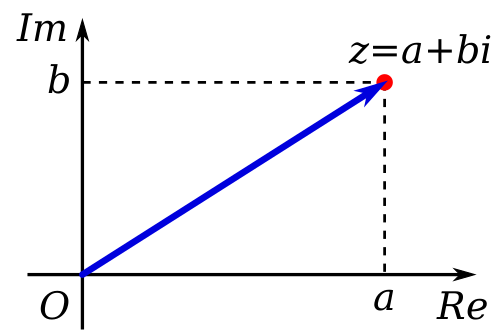
\includegraphics[width=0.7\textwidth]{figures/wiki-complex.png}}


complex conjugates
the complex conjugate of a number typically denoted $\bar{z}$,  for $z = a + ib$ is $\bar{z} = a - ib$, and $\bar{\bar{z}} = z$

Python uses $j$ as the letter to denote imaginary unit, a quick example of basic usage is shown in ADD REF.

\begin{lstlisting}[caption=Basic use of complex numbers in Python syntax]
a = 4 + 6j
b = 0 - 2j
c = a + b 
c 
(4+4j) 
c.conjugate()
(4-4j)
c.real
4.0
c.imag
4.0
np.array(6.5 + 12j)
array(6.5+12.j)
\end{lstlisting}

Complex numbers are used/found/underpin many areas of physics and mathematics, for example they are crucial in the description of quantum mechanical systems, wave optics and Fourier transforms. Consequently, they will be used through this text. 

TODO:
\begin{itemize}
  \item rules for addtion, multiplcation etc.
  \item basic usage
  \item add why they are important and how they are used in this text,
  \item Eulers formula 
  \item replace the diagram with something not from wiki, Should it be interactive?
\end{itemize}



\subsection*{The Fourier Transform, Bandwidth and Nyquist Sampling (CO)}

One of the most important tools in the arsenal of an electron microscopist is the ability to think in reciprocal space, and to mentally convert between real and reciprocal space. By using a TEM, we can easily move between the two spaces, since when we focus parallel electrons down to a point, we convert from an image plane to a diffraction plane. We can also perform this transformation analytically by taking a \emph{Fourier Transform}, or numerically on a computer by using a \emph{discrete Fourier transform}. This is of vital importance for our simulations, as the discrete Fourier transform lies at the heart of all our algorithms for simulating electron scattering. In this text, we will use capital letters to denote reciprocal space functions with variables $(k, \bm{k})$, and lower case letters with variables $(x, \bm{r})$ to denote their real-space counterparts.

The analytic Fourier transform $F(k)$ of a function $f(x)$ can be defined as
\begin{equation}
    F(k)
    =
    \int_{-\infty}^\infty
    f(x)
    \exp\left(
        -2 \ii \pi x k
    \right) dx.
\end{equation}
This transformation can decompose any continuous real-space function into its component frequencies. This transformation can be reversed by taking the \emph{inverse Fourier Transform} given by
\begin{equation}
    f(x)
    =
    \int_{-\infty}^\infty
    F(k)
    \exp\left(
        2 \ii \pi k x
    \right) dk,
\end{equation}
which was first shown by \cite{baron1878analytical}. For all forms of computer simulations, we must perform calculations on a numerical grid with finite sampling. The discrete analog to the Fourier transform $F(k)$ of a function $f(n)$ sampled at integer values of $n$ for a total of $N$ points is given by
\begin{equation}
    F(k)
    =
    \sum_{x=0}^{N-1}
    f(x)
    \exp\left(
        \frac{-2 \ii \pi}{N} x k
    \right),
\end{equation}
and the corresponding inverse transform is given by
\begin{equation}
    f(x)
    =
    \frac{1}{N} \sum_{k=0}^{N-1}
    F(k)
    \exp\left(
        \frac{2 \ii \pi}{N} k x
    \right).
\end{equation}
There are a few remarks worth making about the discrete Fourier transform. The first is that these transformations are implicitly periodic, that is they assume that $f(n)$ repeats an infinite number of times in sequence. Thus if we wish to take a discrete Fourier transform with non-periodic boundary conditions, we will need to pad the function with the appropriate values. The second point is that the forward and inverse transformations differ not only by the sign inside the exponential, but also by the prefactors $(1)$ and $(1/N)$ respectively. This means that typical values of the Fourier transform coefficients will be approximately $N$ times larger than those of the original function. 

Finally, it's also worth noting that we never use the above expressions, since their naive application requires $O(N^2)$. This is "Big O" notation and is a concise description of the time or memory complexity of an algorithm, i.e. in this case how it scales with the number (N) of inputs. Scaling from better to worse; $O(1)$ is constant time e.g. checking a binary number is even or odd,  $O(log(N))$ is logarithmic time e.g. $O(N)$ is linear time e.g. searching unsorted list, $O(Nlog(N))$ loglinear time e.g. FFT, $O(N^2)$ e.g. discrete Fourier transform, ...,  $O(N!)$ is factorial time e.g. brute-force search of travelling salesman. The  multiplication steps of the discrete Fourier transform are too slow to be practical for large vectors or arrays.

Instead, we use a fast Fourier Transform (FFT), which reduces the calculation time to a much more tractable $O(N \log N)$. The first modern FFT algorithm is credited to \cite{cooley1965algorithm}, though its original form appears in the works of Gauss \citep{heideman1985gauss}. A description of this algorithm is beyond the scope of this paper. Many modern implementations of the FFT are available, for example in the FFTW libraries \citep{frigo2005design}. Computing the FFT of a matrix is well suited to GPU acceleration, and is the reason why most modern simulation programs are GPU accelerated, relying on libraries such as cuFFT (ADD REF/CITE). 

\begin{figure}[htbp]
    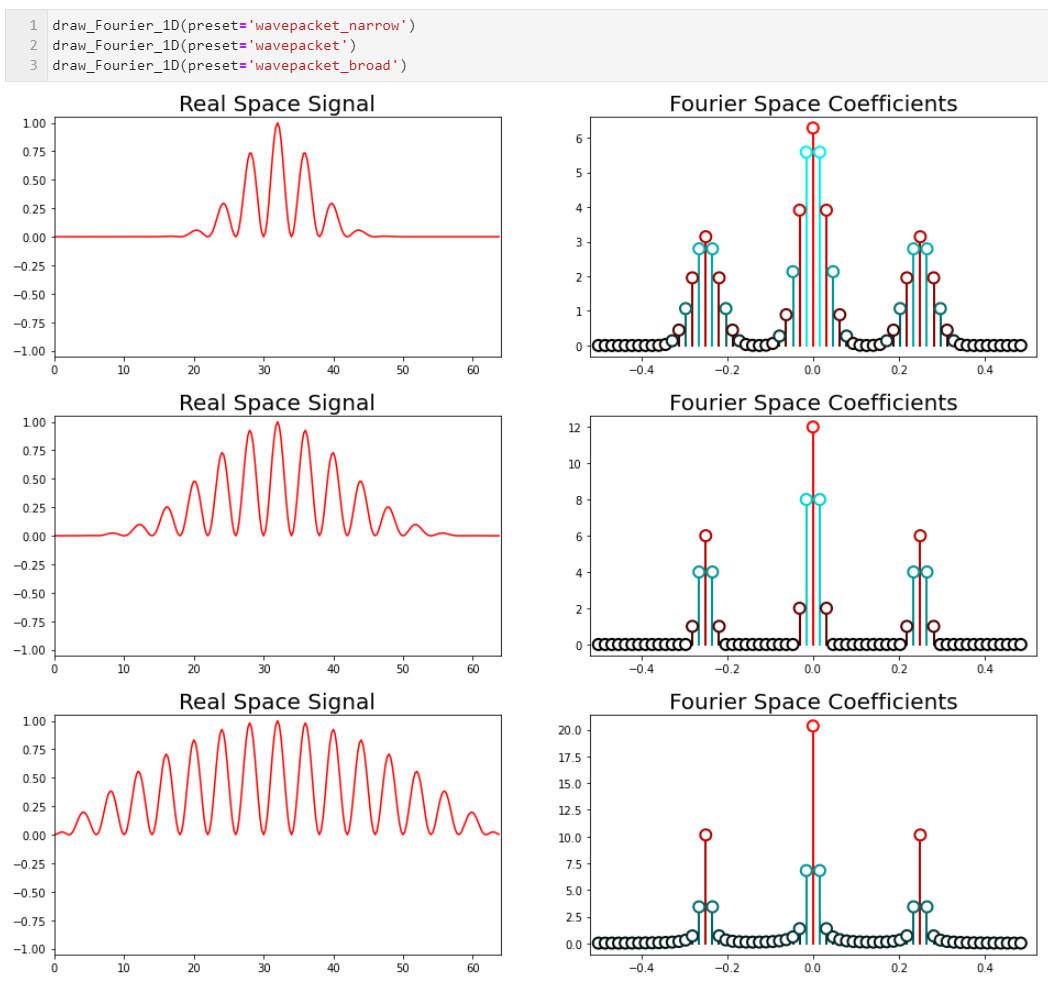
\includegraphics[width=1.0\textwidth]{figures/temp_figure_1D_FFT.png}
    \caption{ Temporary figure for 1D FFT example, \href{https://github.com/tem-elements/tem-elements/blob/main/notebooks/Fourier_Transform_1D.ipynb}{link to current notebook}.}
    \label{vis:1d_fourier}
\end{figure}
%\hl{Colin add text / figure / widget for understanding 1D FFTs}

In STEM simulation, we typically perform simulations of 2D images. Thus we use a 2D FFT, which can be computed by simply taking the FFT along each axis in sequence; the order does not matter due to the orthogonality property of the Fourier transform.

\hl{Colin add text / figure / widget for understanding 2D FFTs}

Bandwidth and FFT, show with widget or figure.
\break
%\begin{lstlisting}[caption=Fourier Transform in Python/numpy]
%array = np.array([[0,1,2],
%                 [3,4,5],
%                 [6,7,8]])
%array
%array([[0, 1, 2],
%       [3, 4, 5],
%       [6, 7, 8]])
%# we can take the FFT of our array. Not the change of data type to a complex type
%fft_array = np.fft.fft2(numpy_array)
%fft_array
%array([[ 36. +0.j        ,  -4.5+2.59807621j,  -4.5-2.59807621j],
%       [-13.5+7.79422863j,   0. +0.j        ,   0. +0.j        ],
%       [-13.5-7.79422863j,   0. +0.j        ,   0. +0.j        ]])
%# we can take the inverse FFT to get our original array back. Although note the data type is still complex. 
%ifft_array = np.fft.ifft2(fft_array)
%ifft_array
%array([[0.+0.j, 1.+0.j, 2.+0.j],
%       [3.+0.j, 4.+0.j, 5.+0.j],
%       [6.+0.j, 7.+0.j, 8.+0.j]])
%\end{lstlisting}

\section*{Physical Concepts (TS)}\label{physics_stuff}

The properties of atoms, molecules and solids are fundamentally determined by quantum mechanics. In this modern theory of physics, some classical concepts such as the electrostatic potential and the propagation of waves are carried over essentially unchanged, whereas many familiar intuitions fail on the level of the very small. In particular, quantum objects including electrons exhibit both wave and particle properties depending on how they are observed -- in the context of electron scattering, matter-wave interference is of central importance. Mathematically, both free propagating electrons and those bound into atoms are described mathematically as complex waves, via so-called electron wavefunctions.

\subsection*{Electron Wavefunctions (TS)}

An electron wavefunction, typically denoted by $\psi$, is a mathematical description of the quantum state of an isolated quantum system. The wavefunctions are complex-valued, and thus not directly observable, but their squared amplitudes can be interpreted as probabilities to find the electrons in particular states that do correspond to physically observable properties of the system. Wavefunctions naturally live in a many-dimensional mathematical space called the Hilbert space. By choosing a basis of representation, they can be represented in real space, typically using either Cartesian (convenient for planewave propagation) or spherical coordinates (convenient for scattering).

Two kinds of wavefunctions are commonly encountered in the context of electron scattering: freely propagating plane and spherical waves, and wavefunctions of electrons bound by (a collection of) atoms. Plane-waves can be mathematically denoted as

\begin{equation}
\psi(\bm{r}, t)=\frac{1}{\sqrt{V}} \mathrm{e}^{i\left(\bm{k} \cdot \bm{r}-\omega t\right)},
\end{equation}

where $\bm{r}$ is the three-dimensional position vector, $t$ is the time, $\bm{k}$ with magnitude $\left|\bm{k}\right|= k = 2 \pi/\lambda$ is the three-dimensional wavevector for wavelength $\lambda$, and $\omega$ is the angular frequency of the wave. $V$ is a volume factor that ensure that integral of the wavefunction over all of space is equal to unity.

Spherical waves can be described similarly,

\begin{equation}
\psi(\bm{r}, t)=\frac{1}{\sqrt{V}} \frac{\mathrm{e}^{i\left(\bm{k}\left|\bm{r}-\bm{r}^{\prime}\right|-\omega t\right)}}{\left|\bm{r}-\bm{r}^{\prime}\right|},
\end{equation}

where $\bm{r}^{\prime}$ now denotes the location of a scattering center, and the denominator $\left|\bm{r}-\bm{r}^{\prime}\right|$ ensures the correct decay of the amplitude as a function of inverse distance.

To describe the propagation of these waves in free space, the imaginary term in the exponential describes periodic variation. Thus for any fixed sum of the spatial and temporal terms in the exponent, the wavefunction has the same value; these represent the planes (or shells) of constant amplitude. To calculate the wave in an arbitrary position, we can simply substitute the new spatial location and time arguments to calculate the resulting amplitude.

\subsection*{Bound Systems: The Schr\"{o}dinger Equation (TS)}

To derive the wavefunction of a bound system, we need to solve the quantum ``equation of motion'' for the electron(s) in the corresponding confining potential: this is the Schr\"{o}dinger equation. The Schr\"{o}dinger equation gives the fundamental mathematical description of quantum systems, describing the time-evolution of their wavefunction. The equation for a single non-relativistic particle can in the position representation be written as

\begin{equation}
    \hbar \frac{\partial}{\partial t} \psi(\bm{r}, t)=\left[-\frac{\hbar^{2}}{2 m} \frac{\partial^{2}}{\partial \bm{r}^{2}}+V(\bm{r}, t)\right] \psi(\bm{r}, t),
    \label{eq:Shrodinger_time}
\end{equation}

where $\hbar$ is the reduced Planck constant, $m$ is the electron mass, and $V(\bm{r}, t)$ is the potential, e.g., Coulomb potential of a nucleus in the case of an atom. Mathematically, the Schr\"{o}dinger equation is linear partial differential equation that assigns a complex number to each point $\bm{r}$ at time $t$, which can be interpreted as the probability amplitude of the electron.

The equation can only be solved analytically for a handful of simple cases, of which the hydrogen atom is an illustrative example. For many such cases, we look for stationary solutions and can thus use the time-independent form the Schr\"{o}dinger equation, written as

\begin{equation}
    \left[-\frac{\hbar^{2}}{2 m} \frac{\partial^{2}}{\partial \bm{r}^{2}}+V(\bm{r})\right] \psi(\bm{r}) = E\psi(\bm{r}),
    \label{eq:Shrodinger}
\end{equation}

where wavefunctions $\psi(\bm{r})$ are the eigenvectors and energies $E$ the eigenvalues of the system.


\subsection*{Electrostatic Potentials (TS)}

The electrostatic potential of a specimen determines not only how the electrons of the system are bound, but also how transmitting electrons scatter via the Lorentz force. It therefore connects the properties of the material to the resulting images or diffraction patterns. The electrostatic potential is fundamentally speaking derived from the electron density of the atoms in a specimen, which is described by their quantum mechanical many-body wavefunction. However, this is only rarely analytically solvable, and various approximations may be needed.

In the case of the hydrogen atom, an analytical solution is possible. To describe the confining effect of the proton of the nucleus on the lone valence electron, we need to include the attractive Coulomb potential in the Hamiltonian. Using the time-independent Schr\"{o}dinger equation, this can be written in spherical coordinates as

\begin{equation}
\left(-\frac{\hbar^{2}}{2 m} \frac{\partial^{2}}{\partial \bm{r}^{2}}-\frac{q_e^2}{4 \pi \varepsilon_{0} r}\right) \psi(r, \theta, \varphi)=E \psi(r, \theta, \varphi),
\end{equation}

where $q_e$ is the elementary charge, $\varepsilon_0$ is the permittivity of free space, $r$ the distance from the nucleus, and $\theta$ and $\varphi$ are respectively the spherical polar and azimuthal angles. The well-known normalizsed solution can be expressed as

\begin{equation}
\psi_{n \ell m}(r, \theta, \varphi)=\sqrt{\left(\frac{2}{n a_0}\right)^{3} \frac{(n-\ell-1) !}{2 n(n+\ell) !}} \mathrm{e^{-\rho / 2}} \rho^{\ell} L_{n-\ell-1}^{2 \ell+1}(\rho) Y_{\ell}^{m}(\theta, \varphi),
\end{equation}

where the quantum numbers ($n$ $\ell$ $m$) numerate the possible states of the electron, $\rho=\frac{2 r}{n a_0}$ with the Bohr radius $a_0=\frac{4 \pi \varepsilon_{0} \hbar^{2}}{m q_e^2}$, and $L_{n-\ell-1}^{2 \ell+1}(\rho)$ is a generalized Laguerre polynomial of degree $n-\ell-1$, and $Y_{\ell}^{m}(\theta, \varphi)$ is a spherical harmonic function of degree $\ell$ and order $m$.

To calculate the electron density, we need to select a set of quantum numbers ($n$ $\ell$ $m$); for the ground state, we can choose $n = 1$, $\ell = m = 0$. The wavefunction thus simplifies to

\begin{equation}
\psi_{1 0 0}(r) = \frac{1}{\sqrt{\pi} a_0^{3 / 2}} \mathrm{e^{-r / a_{0}}},
\end{equation}

whose squared norm gives the (non-relativistic) electron density of hydrogen as

\begin{equation}
\rho(r) = |\psi_{1 0 0}(r)|^2 = \frac{1}{\pi a_0^3} \mathrm{e^{-2 r / a_0}}.
\label{eq:H_density}
\end{equation}

\subsection*{Scattering from a Potential}

To understand how electrons scatter from a potential, we can consider an electron plane wave incident on an isolated atom. The wave interacts with the electrostatic potential of the nucleus and electrons of the atom, and an outgoing spherical wave is generated. To understand the effect of the atom on the wave, we need to calculated the distribution of scattered intensity, which is not isotropic due to the initial linear momentum of the incident wave.

The scattering problem can be formally treated by finding a solution of the Schrödinger equation (Eq.~\ref{eq:Shrodinger}) for the incident electron inside the scattering atom (with electron coordinates $\bm{r^{\prime}}$)

\begin{equation}
    \left[-\frac{\hbar^{2}}{2 m} \frac{\partial^{2}}{\partial \bm{r^{\prime \textmd{2}}}}+V(\bm{r^{\prime}})\right] \psi(\bm{r^{\prime}}) = E\psi(\bm{r^{\prime}}),
\end{equation}

which we can re-write as

\begin{equation}
    \left(\nabla^{2}+k_{0}^{2}\right) \psi\left(\bm{r}^{\prime}\right)=U\left(\bm{r}^{\prime}\right) \psi\left(\bm{r}^{\prime}\right)
\end{equation}

with the substitutions 

\begin{equation}
\begin{aligned} 
    k_{0}^{2} & \equiv \frac{2 m E}{\hbar^{2}}, \\ U\left(\bm{r}^{\prime}\right) & \equiv \frac{2 m V\left(\bm{r}^{\prime}\right)}{\hbar^{2}}.
\end{aligned}
\end{equation}

This can be formally solved with the help of Green's function $G(\bm{r},\bm{r^{\prime}})$ (we refer the reader to \cite{fultz_transmission_2013} for detail) to yield a sum of the incident and scattered components

\begin{equation}
    \psi(\bm{r}) = \psi_{\mathrm{inc}}(\bm{r}) + \psi_{\mathrm{scatt}}(\bm{r}) =
    \mathrm{e}^{\mathrm{i} k_{0} \cdot \bm{r}}+\frac{2 m}{\hbar^{2}} \int V\left(\bm{r}^{\prime}\right) \psi\left(\bm{r}^{\prime}\right) G\left(\bm{r}, \bm{r}^{\prime}\right) \mathrm{d}^{3} \bm{r}^{\prime}.
\label{eq:scattering_schrödinger}
\end{equation}

While this formal solution is in principle exact, it is in the form of an implicit integral equation whose solution $\psi$ appears both inside and outside the integral -- indeed, we have merely transformed the differential Schrödinger equation into an integral equation without solving anything. To proceed, some approximation is needed.

\subsubsection*{Born approximation for electron scattering}

A widely used approximation to solve Eq.~\ref{eq:scattering_schrödinger} is the first Born approximation, whereby we replace the full $\psi$ within the integral simply by the incident planewave. In effect, this approximation makes the assumption that the incident wave is not diminished and scattered only once by the material, which is valid when scattering is weak.

By further assuming that the detector is far from the scatterer, which allows us to work with outgoing planewaves instead of spherical waves, and by aligning the outgoing wavevector $\bm{k}$ with the direction $(\bm{r} - \bm{r^{\prime}})$, as well as assuming that the origin of the coordinate system is near the atom so that $|\bm{r}| \gg |\bm{r^{\prime}}|$, we can write the Green's function as

\begin{equation}
    G\left(\bm{r}, \bm{r}^{\prime}\right) \simeq-\frac{1}{4 \pi} \frac{\mathrm{e}^{i \bm{k} \cdot\left(\bm{r}-\bm{r}^{\prime}\right)}}{|\bm{r}|}.
\end{equation}

By substituting this to Eq.~\ref{eq:scattering_schrödinger} we get

\begin{align}
\psi(\bm{r}) &\simeq \mathrm{e}^{\mathrm{i} k_{0} \cdot \bm{r}}-\frac{m}{2 \pi \hbar^{2}} \int V\left(\bm{r}^{\prime}\right) \mathrm{e}^{\mathrm{i} k_{0} \cdot \bm{r}^{\prime}} \frac{\mathrm{e}^{\mathrm{i} k \cdot\left(\bm{r}-\bm{r}^{\prime}\right)}}{|\bm{r}|} \mathrm{d}^{3} \bm{r}^{\prime}\\
&=\mathrm{e}^{\mathrm{i} k_{0} \cdot \bm{r}}-\frac{m}{2 \pi \hbar^{2}} \frac{\mathrm{e}^{\mathrm{i} \bm{k} \cdot \bm{r}}}{|\bm{r}|} \int V\left(\bm{r}^{\prime}\right) \mathrm{e}^{\mathrm{i}\left(\bm{k}_{0}-\bm{k}\right) \cdot \bm{r}^{\prime}} \mathrm{d}^{3} \bm{r}^{\prime}.
\end{align}

By further defining $\Delta \bm{k} \equiv \bm{k}-\bm{k}_{0}$, we can write the scattered part of the wave as

\begin{equation}
\psi_{\mathrm{scatt}}(\Delta \bm{k}, \bm{r})=\frac{\mathrm{e}^{\mathrm{i} k \cdot \bm{r}}}{|\bm{r}|} f(\Delta \bm{k}),
\end{equation}

which is a function of only the difference between the incident and outgoing wavevectors $\Delta \bm{k}$, describes the change in the direction of the scattered radiation with respect to the incident direction (i.e. momentumn transfer). The factor

\begin{equation}
f(\Delta \bm{k}) \equiv-\frac{m}{2 \pi \hbar^{2}} \int V\left(\bm{r}^{\prime}\right) \mathrm{e}^{-\mathrm{i} \Delta \bm{k} \cdot \bm{r}^{\prime}} \mathrm{d}^{3} \bm{r}^{\prime},\label{eq:formfactor}
\end{equation}

is called the atomic form factor (or electron scattering factor~\cite{kirkland_advanced_2010}) and it describes the angular distribution of scattered intensity. In the first Born approximation it corresponds to the Fourier transform of the scattering potential.% ($f(\Delta \bm{k})=\mathcal{F}_k[V(r)]$).

\subsubsection*{Atomic form factors (TS)}

The atomic form factors thus describe the angular amplitude for scattering of a single electron of by a single atom. While the first Born approximation is  inadequate for describing real specimens (as electrons typically scatter multiple times when passing through a crystal), this description is quite useful since it relates the three-dimensional Fourier transform of the atomic potential to the scattering amplitude.

In the general case, we can describe the potential as a sum of a negative term due to the Coulomb attraction of the nucleus with atomic number $Z$ and a positive term arising from the Coulomb repulsion of the atomic electrons with electron density $\rho(\bm{r})$

\begin{equation}
V(\bm{r})=-\frac{Z e^{2}}{|\bm{r}|}+\int_{-\infty}^{+\infty} \frac{e^{2} \rho\left(\bm{r}^{\prime}\right)}{\left|\bm{r}-\bm{r}^{\prime}\right|} \mathrm{d}^{3} \bm{r}^{\prime}.
\end{equation}

By substituting this into Eq.~\ref{eq:formfactor} and defining a new variable $\bm{R} \equiv \bm{r} - \bm{r}^{\prime}$, so that $\bm{r} = \bm{R} - \bm{r}^{\prime}$ and rearranging, we get

\begin{equation}
f(\Delta \bm{k})=\frac{m Z e^{2}}{2 \pi \hbar^{2}} \int_{-\infty}^{+\infty} \frac{1}{|\bm{r}|} \mathrm{e}^{-\mathrm{i} \Delta k \cdot \bm{r}} \mathrm{d}^{3} \bm{r} -\frac{m e^{2}}{2 \pi \hbar^{2}} \int_{-\infty}^{+\infty} \frac{1}{|\bm{R}|} \mathrm{e}^{-\mathrm{i} \Delta \bm{k} \cdot \bm{R}} \mathrm{d}^{3} \bm{R} \int_{-\infty}^{+\infty} \rho\left(\bm{r}^{\prime}\right) \mathrm{e}^{-\mathrm{i} \Delta \bm{k} \cdot \bm{r}^{\prime}} \mathrm{d}^{3} \bm{r}^{\prime}.
\end{equation}

The two first integrals are simply Fourier transforms of $1/r$ that each yield $4 \pi / \Delta k^2$, giving the general expression for the electron scattering factor of an atom as

\begin{equation}
f(\Delta \bm{k})=\frac{2 m e^{2}}{\hbar^{2} \Delta k^{2}}\left(Z-\int_{-\infty}^{+\infty} \rho(\bm{r}) \mathrm{e}^{-\mathrm{i} \Delta \bm{k} \cdot \bm{r}} \mathrm{d}^{3} \bm{r}\right).
\end{equation}

For kinematic scattering (where diffraction intensity $I(k)=|\psi(k)|^{2}\approx\left|f(k)\right|^{2}$) and within the first Born approximation for electrons (i.e. electron scattering factor is the Fourier transform of the total electrostatic potential) this gives the Mott-Bethe formula for a single atom,

\begin{equation}
f(\Delta \bm{k})=\frac{2 m e^2}{\hbar^{2} \Delta k^{2}} \left(Z-\frac{m c^2}{e^2}f_{x}(\Delta \bm{k})\right),
\end{equation}

relating electron scattering factors with x-ray scattering factors $f_{x}(k)=\mathcal{F}_k[\rho(r)]$, where $\rho(r)$ is the electron density. This comparison highlights that unlike x-ray scattering (where the nucleus is too heavy to accelerate in an interaction with a nearly massless photon), electron scattering is sensitive to both nuclear and electron charges, with the latter contribution being relatively enhanced for small electron scattering angles (corresponding to small momentum vectors $k$). The Mott-Bethe formula is a convenient way to obtain the potential distribution from a charge distribution including the nuclear point charge, effectively by solving Poisson's equation in reciprocal space. 

As an example, we can calculate the x-ray form factor for hydrogen in spherical coordinates (c.f. Eq.~\ref{eq:H_density}), assuming that the incident electron wavevector $\bm{k} = (0, 0, k)$ is parallel to the $z$ axis. In this spherically symmetric case, the x-ray form factor reduces to a radial integral

\begin{equation}
f_\mathrm{x}(\Delta k)=\frac{e^2}{m c^2} \int_{0}^{\infty} \rho(r) \sin (2 \pi \Delta k\, r)\, r\, \mathrm{d}r,
\end{equation}

where the exponential term of the Fourier transform has been expanded as a trigonometric integral. We can calculate the integral explicitly as

\begin{equation}
f_{x}(\Delta k) = \frac{e^2}{m c^2} \int_{0}^{\infty} \frac{r \mathrm{e}^{-2r / a_0}}{\pi a_0^{3}} \sin (2 \pi \Delta k \,r)\, \mathrm{d} r \nonumber
     = \frac{e^2}{m c^2}\frac{1}{\left(1+\pi^2 \Delta k^2 a_0^{2}\right)^{2}}.
\end{equation}

Using the definition of the Bohr radius ($a_{0}=4 \pi \varepsilon_{0} \hbar^{2} / m e^{2}$), the electron scattering factor for hydrogen ($Z = 1$) can then further be written via by the Mott-Bethe formula as 

\begin{equation}
f(\Delta k)=\frac{a_0}{2 \varepsilon_0 \Delta k^{2}} \left(1-\frac{1}{\left(1+\pi^2 \Delta k^2 a_0^{2}\right)^{2}}\right).
\end{equation}

Hydrogen is the only case that is analytically solvable; in general neither the density nor the atomic form factor can be directly written down. Instead, these have been calculated using various approximations to the true multielectron wavefunctions, and tabulated for isolated atoms of all elements as isolated atomic potentials.

\subsection*{Isolated Atomic Potentials (TS)}

Since the Schrödinger equation cannot be solved analytically even for most molecules, let alone solid-state systems, several kinds of approaches have been developed to obtain approximate solutions. These accurate but computationally very expensive techniques have been used to parametrize what are called isolated atomic potentials -- or, equivalently in reciprocal space, electron scattering factors -- which describe the potential of a specimen as a sum of isolated, non-interacting atom potentials. This approximation is often called the independent atom model.

A potential parametrization is a numerical fit to such first principles calculations of electron atomic form factors that describe the radial dependence of the potential for each element. One of the most widely used parametrizations is the one published by \cite{kirkland_advanced_2010}, who fitted Dirac-Fock scattering factors with combination of Gaussians and Lorentzians. In 2014, Lobato and Van Dyck improved the quality of the fit further, using hydrogen's analytical non-relativistic electron scattering factors as basis functions to enable the correct inclusion of all physical constraints~\cite{lobato_accurate_2014}.

An interactive example of independent-atom scattering potentials for elements up to $Z = 32$ is shown below (the code can be found on \href{https://github.com/jacobjma/hands-on-guide-to-TEM-simulations/blob/main/notebooks/toma/Atomic_potentials.ipynb}{GitHub}).

\framebox(468,280){
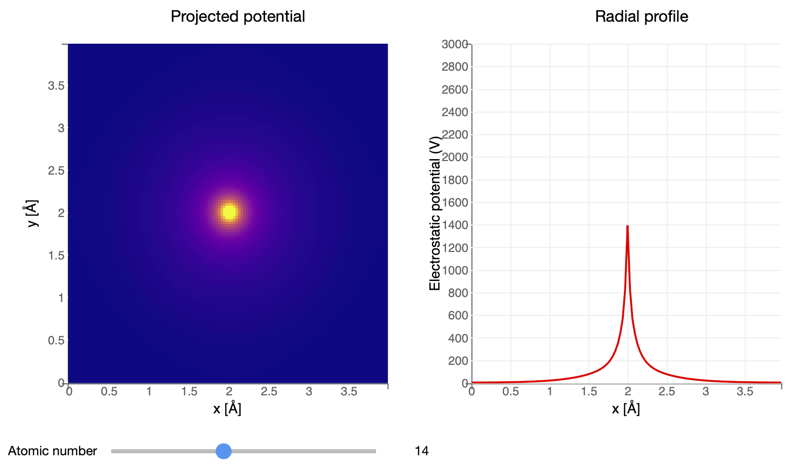
\includegraphics[width=1\textwidth]{figures/Atomic_potentials_widget.png}}

\subsection*{Density Functional Theory Potentials (TS)}

Since the complicated many-body interactions of multiple electrons mean that wavefunction cannot in general be analytically solved, further approximations are needed. Density functional theory (DFT) is the most prominent one, and is widely use for modeling the electronic structure of molecules and solids. In DFT, the combinatorially intractable many-body problem of $N$ electrons with $3N$ spatial coordinates is reduced to a solution for the three spatial coordinates of the electron density that can be variationally reached. This approximation would in principle be exact, but a term that describes electron exchange and correlation is not analytically known and must be approximated.

Although the ground-state electron density for all electrons, including those in the core levels and in the valence, can in principle be solved within the DFT framework, the electron wavefunctions rapidly oscillate near the nuclei, making a numerical description computationally very expensive. To make calculations practical, some partition of the treatment of the cores and the valence is therefore typically needed. Pseudopotential~\cite{schwerdtfeger_pseudopotential_2011} and projector-augmented wave (PAW) methods~\cite{blochl_projector_1994} have in recent years matured to offer excellent computational efficiency. The core electrons are not described explicitly in either method, but in the former are replaced by a smooth pseudo-density, while in the latter, by smooth analytical projector functions in the core region.

Inverting the projector functions allows the exact core electron density to be analytically calculated, making the PAW method arguably ideally suited for efficient and accurate \textit{ab initio} all-electron electrostatic potentials. The PAW method is accordingly the approach chosen for \textsc{abTEM}, specifically via the grid-based DFT code \textsc{GPAW} (more details on the method can be found in the literature~\cite{blochl_projector_1994,enkovaara_electronic_2010}). Notably for our purposes here, GPAW allows the full electrostatic potentials (with smeared nuclear contributions) to be efficiently calculated for molecules and solids, and seamlessly used for electron scattering simulations using \textsc{abTEM}.

To come back to our hydrogen example, we can analytically calculate its full electrostatic potential by solving the Poisson equation for the charge density of the electron (charge $-q_e$) combined with the Coulomb potential of the nucleus ($+q_e$). The Poisson equation is

\begin{equation}
\nabla^{2} V(r) = -\frac{4\pi}{\varepsilon_0} \left(-q_e \rho(r) + q_e \delta(r)\right),
\end{equation}

with the solution

\begin{equation}
V(r) = \frac{q_e}{4 \pi \epsilon_{0}} \frac{\mathrm{e^{-2 r / a_0}}}{r}\left(1 + \frac{r}{a_0}\right).
\label{eq:H_potential}
\end{equation}

This expression is singular at the origin due to the point charge of the nucleus, but that singularity gets smeared out due and numerically discretized in practical calculations (by default, GPAW smears the nuclear potentials with a Gaussian function).

In Fig.~\ref{fig:H_atom}, we plot the exact solution of Eq.~\ref{eq:H_potential} against the Kirkland IAM parameterization as well as a GPAW calculation (the code can be found on \href{https://github.com/jacobjma/hands-on-guide-to-TEM-simulations/blob/main/notebooks/toma/H_atom.ipynb}{GitHub}).. While all models agree perfectly near the nucleus (the discontinuous appearance of the line is due to a finite computational grid with a spacing of 0.02~\AA), where the potential is the strongest, small differences emerge further away. In the case of the DFT model, the simulation box is finite in size, and thus the continuity requirement of the wavefunction and corresponding density slightly affect the long-range part of the calculated potential. The choice of exchange-correlation functional may also slightly influence the results.

\framebox(468,130){
    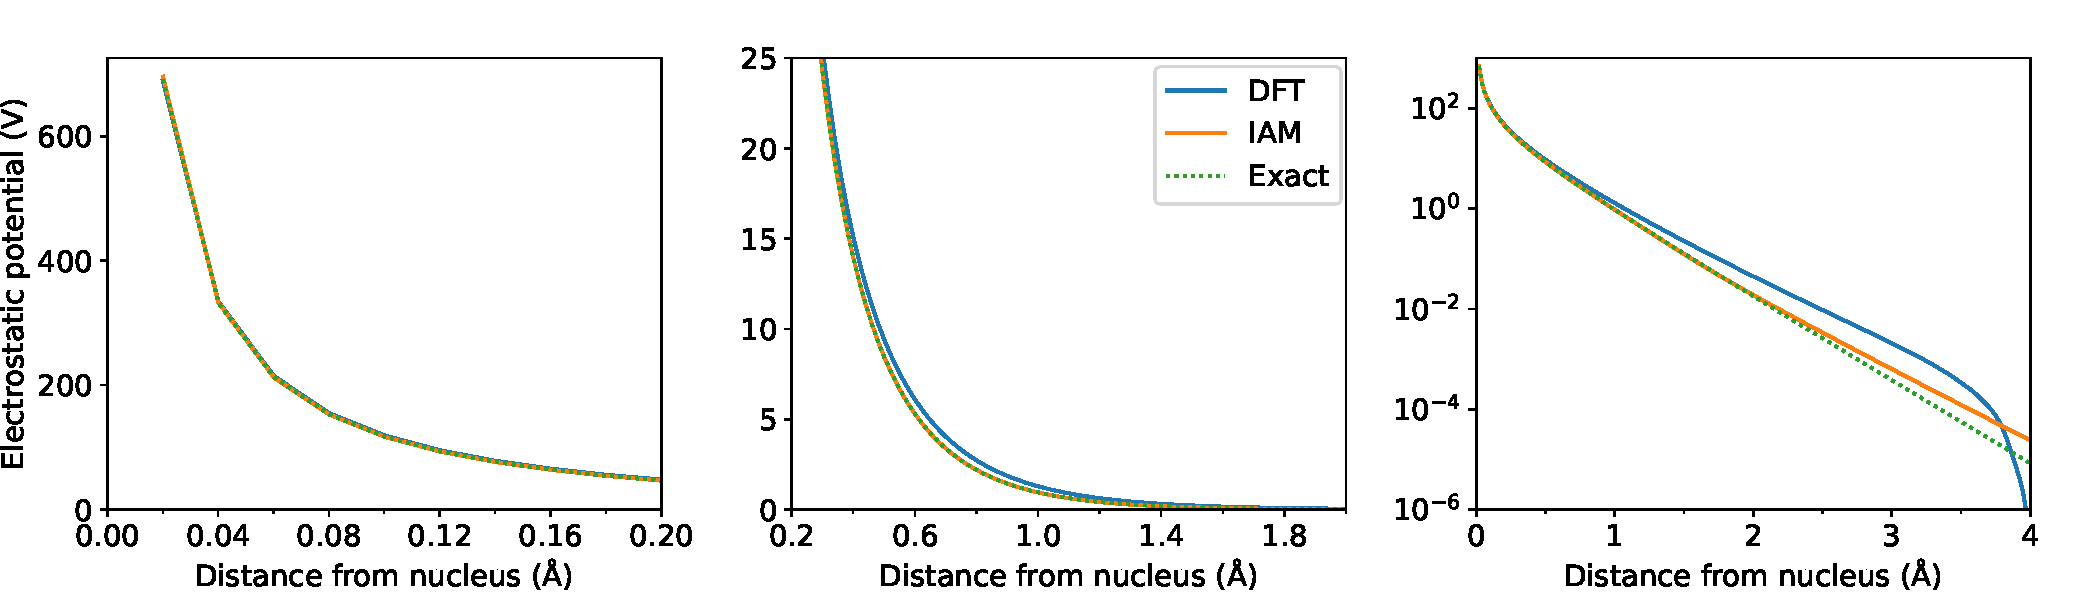
\includegraphics[width=1\textwidth]{figures/H_atom.pdf}
    \label{fig:H_atom}
}

Although IAM potentials are useful for many purposes, they do neglect chemical bonding, which may be measurable and of interest. To illustrate this difference, an interactive comparison of the IAM and DFT scattering potentials of the H$_2$ molecule at different distances between the H atoms is shown below (the code can be found on \href{https://github.com/jacobjma/hands-on-guide-to-TEM-simulations/blob/main/notebooks/toma/H2_molecule.ipynb}{GitHub}).

\framebox(468,300){
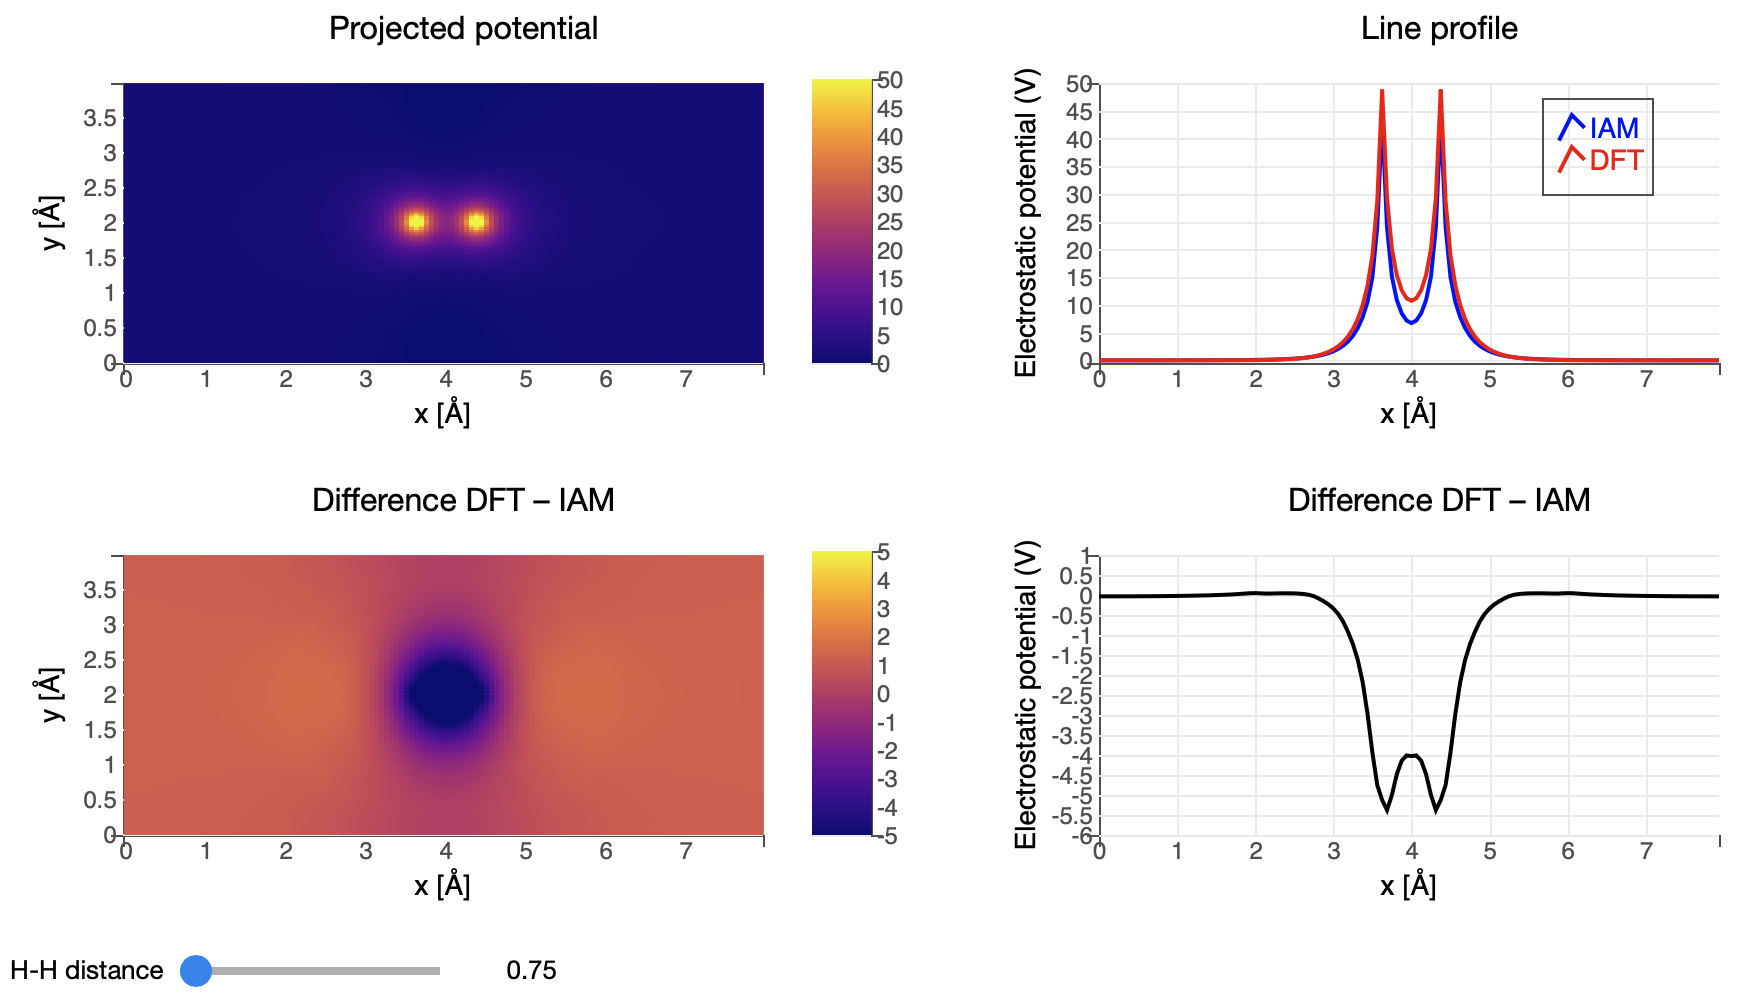
\includegraphics[width=1\textwidth]{figures/H2_molecule_widget.png}}

\subsection*{Numerical Solutions of the Schr\"{o}dinger Equation (CO)}

As discussed previously, the Schr\"{o}dinger equation typically cannot be solved analytically in complex systems. Therefore, in order to perform electron scattering simulations, we must calculate numerical solutions of Eq.~\ref{eq:Shrodinger_time} for electron waves. First, we define the \cite{debroglie1925recherches} wavelength of a free electrons (corrected for relativistic effects) as
\begin{equation}
    \lambda = \frac{h \, c}{\sqrt{e \, E_0 (2 \, m \, c^2 + e \, E_0)}},
    \label{eq:wavelength}
\end{equation}
where $h$ is the Plank constant, $c$ is the speed of light, $e$ is the electron charge, and $E_0$ is the accelerating voltage applied to the electron. Using SI units for Eq.~\ref{eq:wavelength} will give the wavelength in units of meters. In practice we typically use length units of \angstroms{} for all calculations, and therefore multiple this result by $10^{10}$.

Next, we define the electron-potential interaction constant as (the numerical values of these constants can be found in Appendix~\ref{app:constants})
\begin{equation}
    \sigma = \frac{2 \pi \, m \, e \, \lambda}{h^2}.
    \label{eq:interaction_constant}
\end{equation}

In our simulations, we will assume the $z$-position coordinate of the wavefunction $\psi(\bm{r})$ is alone sufficient to describe its propagation in both time and space, and therefore drop the $t$ coordinate. Substituting Eqs.~\ref{eq:wavelength} and \ref{eq:interaction_constant} into Eq.~\ref{eq:Shrodinger_time}, we obtain \citep{kirkland2020}
\begin{equation}
    \frac{\partial }{\partial z} \psi(\bm{r})
    =
    \frac{\ii \lambda}{4 \pi} {\nabla_{xy}}^2 \psi(\bm{r})
    + 
    \ii \sigma V(\bm{r}) \psi(\bm{r}),
    \label{eq:Shrodinger_electron}
\end{equation}
where ${\nabla_{xy}}^2 = \partial^2/\partial x^2 + \partial^2/\partial y^2$. This equation shows the overall numerical recipe we will use; when the wavefunction $\psi_0(\bm{r})$ is at position $z_0$, we will evaluate the operators on the right hand side over a distance $\Delta z$ to calculate the new wavefunction $\psi(\bm{r})$ at position $z_0 + \Delta z$. \cite{kirkland2020} gives the formal operator solution to Eq.\ref{eq:Shrodinger_electron} as
\begin{equation}
    \psi(\bm{r})
    = 
    \exp \left\{
    \int_{z_0}^{z_0 + \Delta z} 
    \left[
        \frac{\ii \lambda}{4 \pi} {\nabla_{xy}}^2
        + 
        \ii \sigma V(\bm{r})
    \right] dz
    \right\}
    \psi_0(\bm{r})
    \label{eq:Shrodinger_solution}
\end{equation}
Assuming $\Delta z$ is small, Eq.~\ref{eq:Shrodinger_solution} can be simplified to
\begin{equation}
    \psi(\bm{r})
    = 
    \exp\left[
        \frac{\ii \lambda}{4 \pi} \Delta z {\nabla_{xy}}^2
        + 
        \ii \sigma V_{\Delta z}(\bm{r})
    \right]
    \psi_0(\bm{r})
    \label{eq:Shrodinger_simple}
\end{equation}
where
\begin{equation}
    V_{\Delta z}(\bm{r})
    =
    \int_{z_0}^{z_0 + \Delta z} 
    V(\bm{r}) dz,
\end{equation}
is a thin slice of the potential. Unfortunately, even with the above approximations, Eq.~\ref{eq:Shrodinger_simple} cannot be solved in closed form due to the two non-commuting operators. Instead, we will solve it numerically by using a split-step method, where we calculate solutions for each operator independently, and alternating their application  to the electron wavefunction. This solution was introduced by \cite{cowley1957scattering} and is known as the multislice method.


\subsection*{Free Space Wave Propagation}

For an electron wavefunction moving through free space, we can set $ V_{\Delta z}(\bm{r}) = 0$. This assumption and our ability to split the $x$ and $y$ derivatives into two terms, allows us to simplify Eq.~\ref{eq:Shrodinger_simple} to 
\begin{eqnarray}
    \psi(\bm{r})
    &=& 
    \exp\left[
        \frac{\ii \lambda}{4 \pi} \Delta z {\nabla_{xy}}^2
    \right]
    \psi_0(\bm{r}) 
    \nonumber \\
    &=& 
    \sum_{n=0}^\infty
    \frac{1}{n!}
    \left(
        \frac{i \lambda \Delta z}{4 \pi}
    \right)^n
    \sum_{m=0}^n
    {n \choose m}
    \left(
        \frac{\partial}{\partial x}
    \right)^{2n-2m}
    \left(
        \frac{\partial}{\partial y}
    \right)^{2m}
    \psi_0(\bm{r}).
\end{eqnarray}
This expression looks complicated due to the infinite series of derivatives, but we can solve it by taking the 2D Fourier transform of both sides, where the Fourier space wavefunction is defined as $\Psi(\bm{k}) = \FFT\{\psi(\bm{r})\}$ and where both $\bm{r}$ and $\bm{k}$ from here onward are 2D variables within the plane perpendicular to the propagation direction. This solution gives
\begin{eqnarray}
    \Psi(\bm{k})
    &=&
    \sum_{n=0}^\infty
    \frac{1}{n!}
    \left(
        \frac{i \lambda \Delta z}{4 \pi}
    \right)^n
    \sum_{m=0}^n
    {n \choose m}
    \left(
        2 \pi \ii k_x
    \right)^{2n-2m}
    \left(
        2 \pi \ii k_y
    \right)^{2m}
    \Psi_0(\bm{k})
    \nonumber \\
    &=&
    \sum_{n=0}^\infty
    \frac{1}{n!}
    \left(
        - \ii \pi \lambda \Delta z
    \right)^n
    \sum_{m=0}^n
    {n \choose m}
    {k_x}^{2n-2m}
    {k_y}^{2m}
    \Psi_0(\bm{k})
    \nonumber \\
    &=&
    \sum_{n=0}^\infty
    \frac{1}{n!}
    \left[
        - \ii \pi \lambda \Delta z
        ({k_x}^2 + {k_y}^2)
    \right]^n
    \Psi_0(\bm{k})
    \nonumber \\
    &=& \exp\left(
        - \ii \pi \lambda  \Delta z |\bm{k}|^2
    \right)
    \Psi_0(\bm{k}).
\end{eqnarray}
Thus we can calculate the propagation of an electron wave through free space over a distance $\Delta z$ by taking the Fourier transform, multiplying each pixel by the above free space propagation operator, and taking the inverse Fourier transform.

\hl{Colin section 1}  - adapt my wave propagation movies into interactive demos

\framebox(468,50){\hl{CODE BLOCK - plane wave propagation}}

\hl{Colin section 2}  - adapt my wave propagation movies into interactive demos (I think I've done this for at least a couple of your functions AMR)

\subsection*{Constructive and Destructive Interference}


\section*{Simulating Electron Scattering}\label{electron_sacttering}


\subsection*{The Multislice Algorithm for S/TEM Simulation}

\begin{figure}[h]
    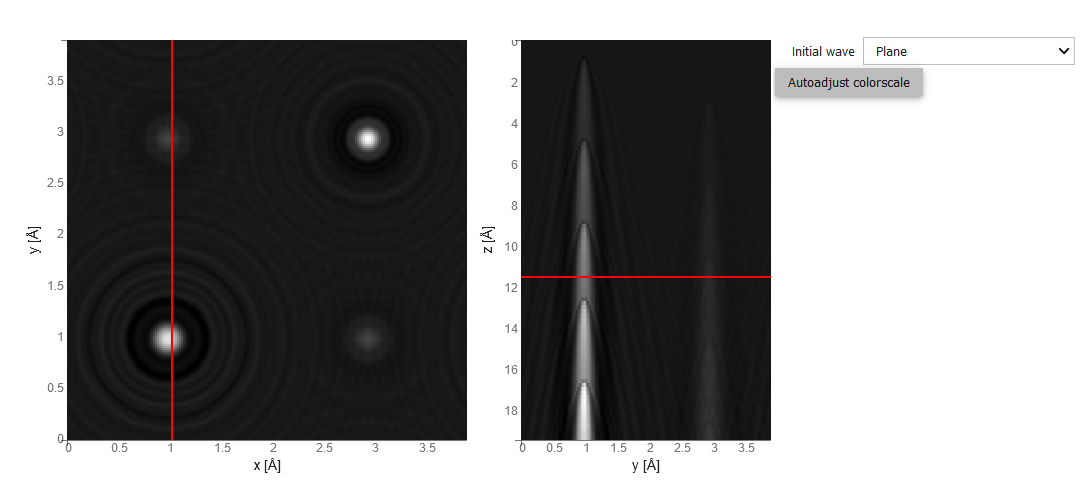
\includegraphics[width=1\textwidth]{figures/3d_wavefunction.png}
    \caption{ \href{https://tem-elements.herokuapp.com/voila/render/notebooks/3D_wavefunction.ipynb}{(Link to visualization)}}
    \label{vis:3d_wavefunction}
\end{figure}

\subsection*{The PRISM Algorithm for STEM Simulation}

% Extensions of PRISM?
% \subsection*{Partitioned PRISM for STEM Simulation}

We probably want a section where we make STEM probes interactively - a few ideas:
-probe size vs parameters (AMR)
-probe size for specialized shapes like phase plates or amplitude plates / bullseye probes
-Recent user question - how do I define probe overlap in ptychography?  I use ``shared intensity'' vs probe spacing, i.e sum(int1 * int2) / sqrt(sum(int1**2) * sum(int2**2)) - this would be a neat interactive demo 


\section*{Simulation Inputs and Parameters}\label{sim_inputs}

\subsection*{Building Scenes from Atomic Coordinates}
The first step of an image simulation is creating a representation of the sample. For most simulations this is achieved by building the object from its constituent atoms. In its most basic form the position in 3D space and type of each atom must be defined, additionally it is typical to include partial occupancy and Debye-Waller factor (DWF). Once the object is created, it must be passed to the simulation in an parsable way. There are an innumerable ways of doing this, and multiple bespoke file formats which in theory are all interchangeable. The most common/universal file types are \emph{.xyz}, and and \emph{.cif}. With \emph{.xyz} being the simpler of the two, defining the cell (size and angles) of the entire object, and atom type, x, y, z, and  occupancy and DWF for every atom in the object. Whereas, \emph{.cif}, describes the unit cell, and the symmetry operations to tile the unit cell, which can be a much more efficient representation for highly symmetric objects, but will result in the same length file for non symmetric objects. 

 



%\newline
\emph{The \emph{.cif} file format is widely used in x-ray crystallography.}

\textbf{TODO}: 
\begin{itemize}
    \item add way to view the atoms
    \item translating between file formats, pymatgen/ASE
    \item add short example of .xyz
    \item add short example of .cif
\end{itemize}

\subsubsection*{Making simple samples (TS)}

e.g. Single Nanoparticles, Simple structures from materials project, CIF files etc. 

1) Searching  materials repositories such as, \href{https://materialsproject.org}{Materials Project}, \href{http://rruff.geo.arizona.edu/AMS/amcsd.php}{American Mineralogist Crystal Structure Database} ... and downloading the corresponding structure file. 
\newline
2) Structures with easily defined and periodic lattices such as graphene, TMDCs, nanoribbons, and (metallic) nanoparticles can be created using easily be created using python libraries such as \href{https://wiki.fysik.dtu.dk/ase/}{Atomic Simulation Environment (ASE)}, \href{https://pymatgen.org/#}{pymatgen}. 





\subsubsection*{Making simple samples more realistic}

\begin{figure*}[htbp]
    \centering
    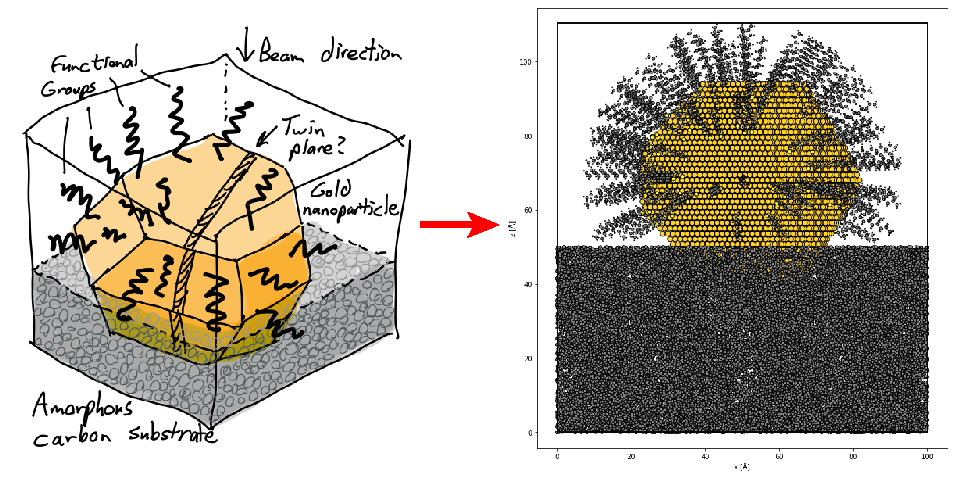
\includegraphics[width=4.0
    in]{figures/complex_structure.pdf}
    \caption{{\bf Generating more complex simulation cells} - \href{https://github.com/tem-elements/tem-elements/blob/main/notebooks/Sample_NP_functionalized_substrate.ipynb}{link to notebook}}
    \label{Fig:sample_NP_func_substrate}
\end{figure*}

Often we will perform simulations of simple model systems to better understand the image contrast in TEM or STEM. One example of a such as a system is a ``nanoparticle floating in space'' geometry. For nanoparticles which contain high atomic number atoms and rest on a thin substrate, this can be a reasonable approximate. However, we often wish to perform more realistic simulations. The simplest addition is to add a substrate to our simulation cell. This notebook in Fig.~\ref{Fig:sample_NP_func_substrate} will walk you through the process of using ASE to create a nanoparticle with an internal twin boundary defect, adding some randomly positioned surface functionalization molecules, and then placing the particle onto an amorphous carbon substrate.

The first step is to define our atomic structure. For this example, we use the face centered cubic (fcc) Au structure. Next, we tile the Au lattice to fill a Gibbs-Wulff \citep{wulff1901question} polyhedron. The basic idea behind the Gibbs-Wulff construction is that the various crystallographic surfaces of a nanoparticle have normal vector distances from the particle origin which scale proportionally with the surface free energy. This is a good approximation for particles in solution. However, \cite{winterbottom1967equilibrium} shows that it can be improved by including the substrate-particle interfacial energy or the energies of any internal planar defects such as grain boundaries in the equilibrium shape calculation. Thus we can easily define most nanoparticles by simply specifying the number of planes or vector normal distances for a small number of facets, as we do here.

To introduce a twin defect, we could mirror the particle about a [1,1,1] close-packed plane, or perform a rotation about the [1,1,1] vector for all atoms on one side of the twin. We have opted for the second solution, as outlined in the notebook. Finally we rotate the particle to a (0,1,1) zone axis in order to easily image the twin boundary, mirroring the tilting we might perform in a real experiment.

Next, we position some functional groups onto random positions on the nanoparticle surface. We have selected a thiolate structure,  obtained from \cite{yang2007synthesis}. 

The last structural component we need is the amorphous carbon substrate. We have opted to use the realistic amorphous carbon models published by cite{ricolleau2013random}. First, we import the block of carbon, which measures 5x5x5 nanometers in size.  This is too small to use for our nanoparticle which is roughly 5 nm in diameter, and so we tile the amorphous carbon block 2 times in both the x and y directions. Because the structure already has 3D periodicity, we can safely tile in any direction. If we needed to further randomize the structure, we could apply a random tilt and then crop the desired surfaces. Our next step is to position the substrate directly below the particle, and then remove any overlapping atoms, defined as those within a distance of 3 $\rm{\AA}$. Finally, we recompute the cell boundaries to hold the periodic structure in x and y and provide sufficient distance along the beam direction z to contain all atoms.






\subsubsection*{Making complex structures (CO)}
e.g. some materials with different strains, boundaries, domain walls etc. 

Relax grain boundary structure using EMT in ASE?





\subsubsection*{Making soft-matter samples}
e.g. proteins or polymers

Read in PDB file using ASE, make cell, add vitreous ice possibly (or continuum water model from Shang and Sigworth)


%\subsubsection*{Importing an MD trajectory}

\subsubsection*{Common mistakes/errors}
Boundaries when tiling 
Unit cells too small/wrap around errors



\subsection*{Wavefunction Sampling}




\subsection*{Wave Aberrations}

An ideal lens forms a spherical wave converging on or emerging from a single point. This means that a plane wave will be converted to a spherical wave converging at the focal point of the lens, and the image of a point source is also a point. In STEM we want the objective lens to produce the smallest possible probe and in HRTEM we want the objective lens to produce a perfect magnified image of the sample. Both of these objectives require that we minimize all aberrations (except for defocus) as much as possible. 

However, while the last decades has seen enormous improvements in the optics of electron microscopes, they are far from ideal optical system. Imperfections causes the focused wave front to deviate from the ideal spherical surface. 

This deviation is typically expressed as a phase error, $\chi(\bm{k})$. Given a Fourier space wavefunction $\Psi_0(\bm{k})$ entering the lens, the wavefunction after passing through that lens can thus be expressed as 
\begin{align*}
    \Psi(\bm{k}) = \Psi_0(\bm{k}) \mathrm{e} ^ {-i \chi(\bm{k})}.
\end{align*}

Another, possibly more intuitive way of framing the phase error is the point spread function 
\begin{align*}
    \mathrm{PSF}(\bm{r}) = \FFT \mathrm{e} ^ {-i \chi(\bm{k})} ,
\end{align*}
the point spread function describes how an imaging system responds to a point source. In STEM, the PSF would be the image of the probe, given an infinite objective aperture, in HRTEM the PSF would be how a perfect point source is imaged by an objective lens with an infinite collection angle.  

The phase error can be expressed in different ways, however, it is traditionally written as a series expansion. One popular choice is to write it as an expansion in polar coordinates
\begin{align*}
    \chi(k, \phi) = \frac{2 \pi}{\lambda} \sum_{n,m} \frac{1}{n + 1} C_{n,m} (k \lambda)^{n+1} \cos\left[m (\phi - \phi_{n,m}) \right] ,
\end{align*}
where $k$ is the Fourier space radial coordinate and $\phi$ is the corresponding azimuthal coordinate. The coefficient $C_{n,m}$ represents the magnitude of an aberration and $\phi_{n,m}$ gives a direction to that aberration. There are other ways of representing the aberration function, you might have seen the Cartesian representation where some parameters has an "a" and "b" version.

As a special case, if the microscope is well-aligned the non-symmetric components might be small. Then the contrast transfer function can be expressed more simply
\begin{align*}
    \chi(k) \approx \frac{2\pi}{\lambda}\left( \frac{\lambda^2 k^2}{2} \Delta f + \frac{\lambda^4 k^4}{4} C_s \right) \quad ,
\end{align*}
here we used the common aliases of the aberration coefficients, so $C10 = -\Delta f$ is the negative defocus and $C_{30} = C_s$ is the third order spherical aberration. Table ?? shows how other aberration coefficients matches with the well-known aberration aliases.  

You can explore how aberrations affect the contrast transfer function in visualization \ref{}

\hl{CO - love the vis idea of course, we could also add one for HRTEM where we demonstrate that for a weak phase object (a protein?) there is no contrast, so you need some aberration (or a phase plate) to see anything! }





\begin{figure}[h]
    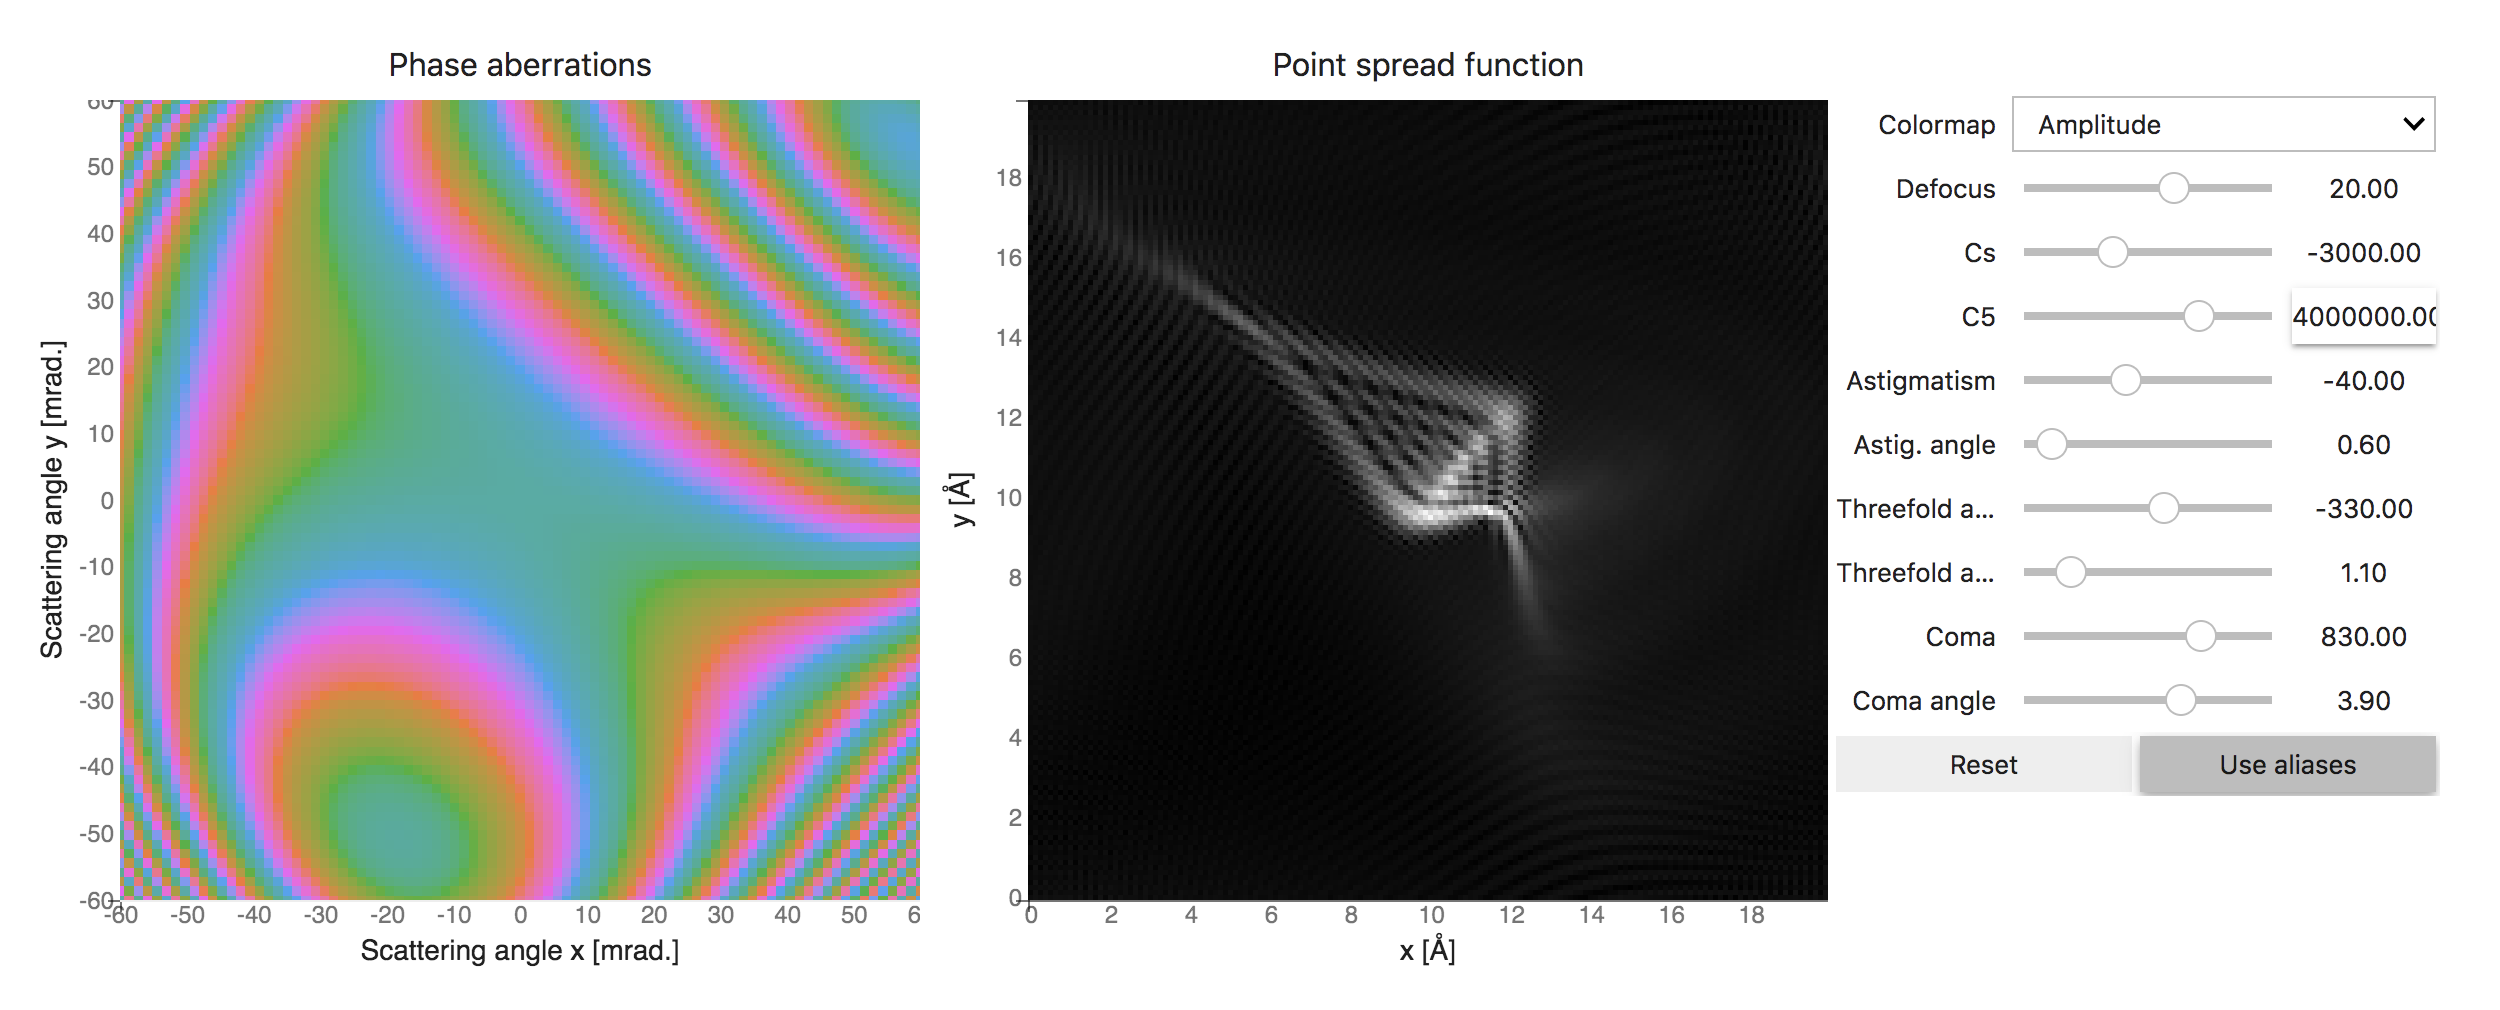
\includegraphics[width=1\textwidth]{figures/aberrations_and_psf.png}
    \caption{\href{https://tem-elements.herokuapp.com/voila/render/notebooks/Aberrations.ipynb}{(Link to visualization)}}
\end{figure}





%From quantum mechanics we know that it is not possible, given a lens with a finite aperture, to focus electrons to a single point, instead we say that ideal (electron-)optical systems are diffraction limited. 


\subsection*{Other Microscope and Detector Parameters}

\section*{TEM Simulations with Plane Waves}\label{TEM_SIMS}

\subsection*{Imaging}

\subsection*{Diffraction}

\subsection*{Biological Samples Embedded in Ice}

\section*{Including Limited Coherence}

\begin{figure}[h]
    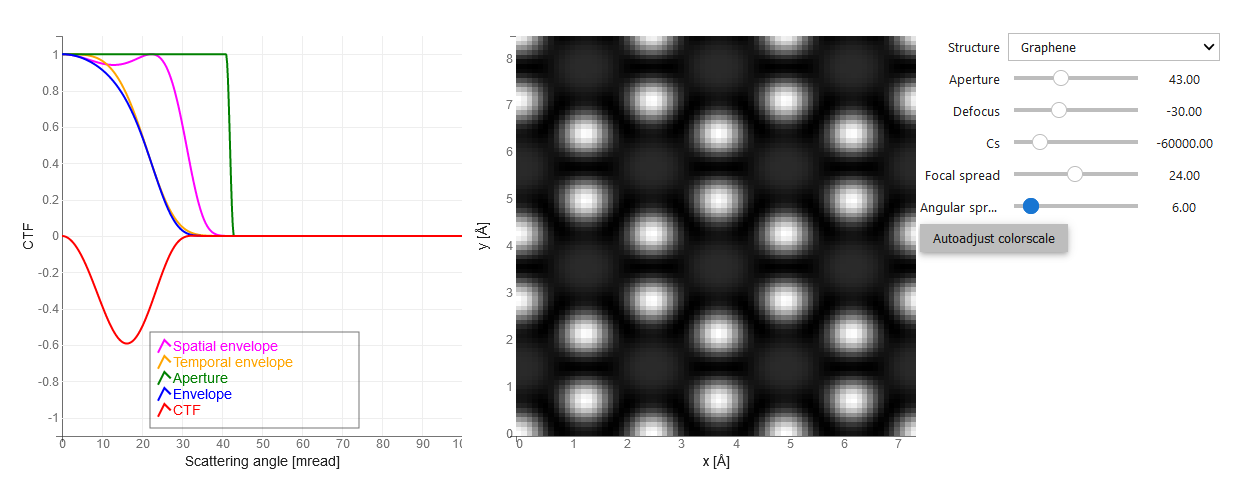
\includegraphics[width=1\textwidth]{figures/hrtem.png}
    \caption{\href{https://boiling-wildwood-85903.herokuapp.com/voila/render/hrtem.ipynb}{(Link to visualization)}}
\end{figure}

\begin{figure}[h]
    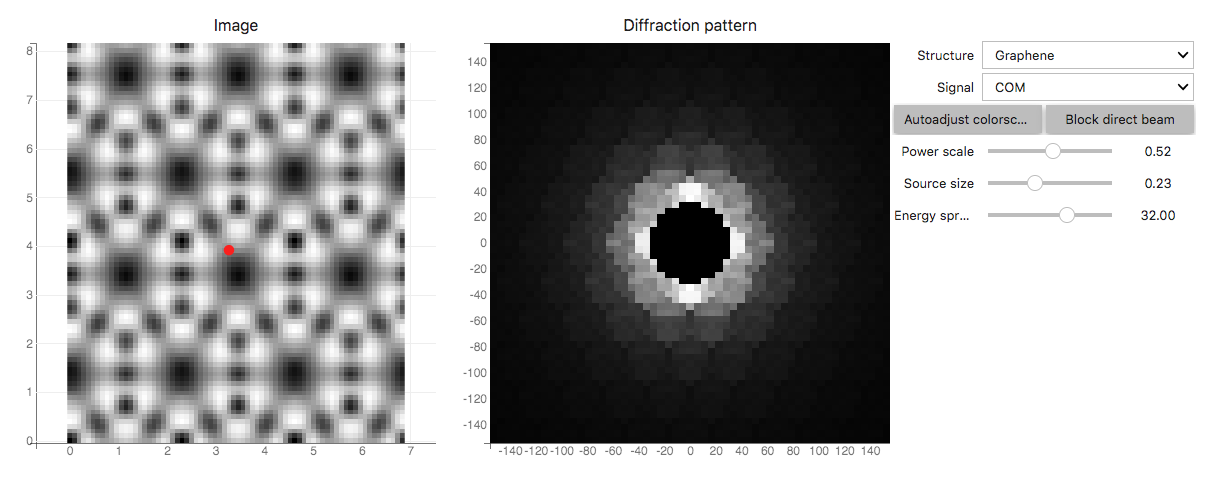
\includegraphics[width=1\textwidth]{figures/limited_coherence_STEM.png}
    \caption{\href{https://tem-elements.herokuapp.com/voila/render/notebooks/limited_coherence_STEM.ipynb}{(Link to visualization)}}
\end{figure}



\section*{STEM Simulations with Converged Probes}\label{STEM_SIMS}

\subsection*{Initial Conditions of the Electron Wave}
In STEM the objective lens acts on the electron beam before the beam reaches the specimen, hence the effects of the lens aberrations and aperture is incorporated in the initial conditions of the wavefunction.

The incident probe wavefunction is easiest to define in Fourier space
\begin{align} \label{eq:fourier_probe}
    \Psi_0(\bm{k}) = A(\bm{k}) \mathrm{e}^{-i\chi(\bm{k})},
\end{align}
where the amplitude, $A(\bm{k})$, is the aperture function and the phase, $\chi(\bm{k})$, is the aberration function introduced in section \ref{}. The aperture is usually a disk with a radius given by the cutoff semiangle
\begin{align}
    A(\bm{k}) = 
    \begin{cases}
    1, &  \lambda k = \alpha < \alpha_{cutoff} \\
    0,              & \text{otherwise} .
    \end{cases}
\end{align}
While the above definition is typical for most STEM experiments, the initial wavefunction can be defined using any other complex function and other initial conditions may be required for simulating more exotic experiments such phase plate STEM.

The probe is transferred to the specimen using an inverse Fourier transform and, in the same step, we can shift the by the Fourier shift theorem
\begin{align} \label{eq:realspace_probe}
    \psi_0(\bm{r}, \bm{r}_p) = \mathcal{F}_{\bm{q}}^{-1} \left[\mathrm{e^{-i\chi(\bm{k}) - 2 \pi i \bm{k}\cdot \bm{r}_p }} A(\bm{k}) \right] ,
\end{align}
where, $\bm{r}_p$, is a specified probe position in relative to the atomic coordinates.

In Vis. \ref{vis:probe}, we present an interactive visualization for exploring the relationship between size and shape of the incident probe and some parameters of the aperture and aberration functions.

\begin{figure}[h]
    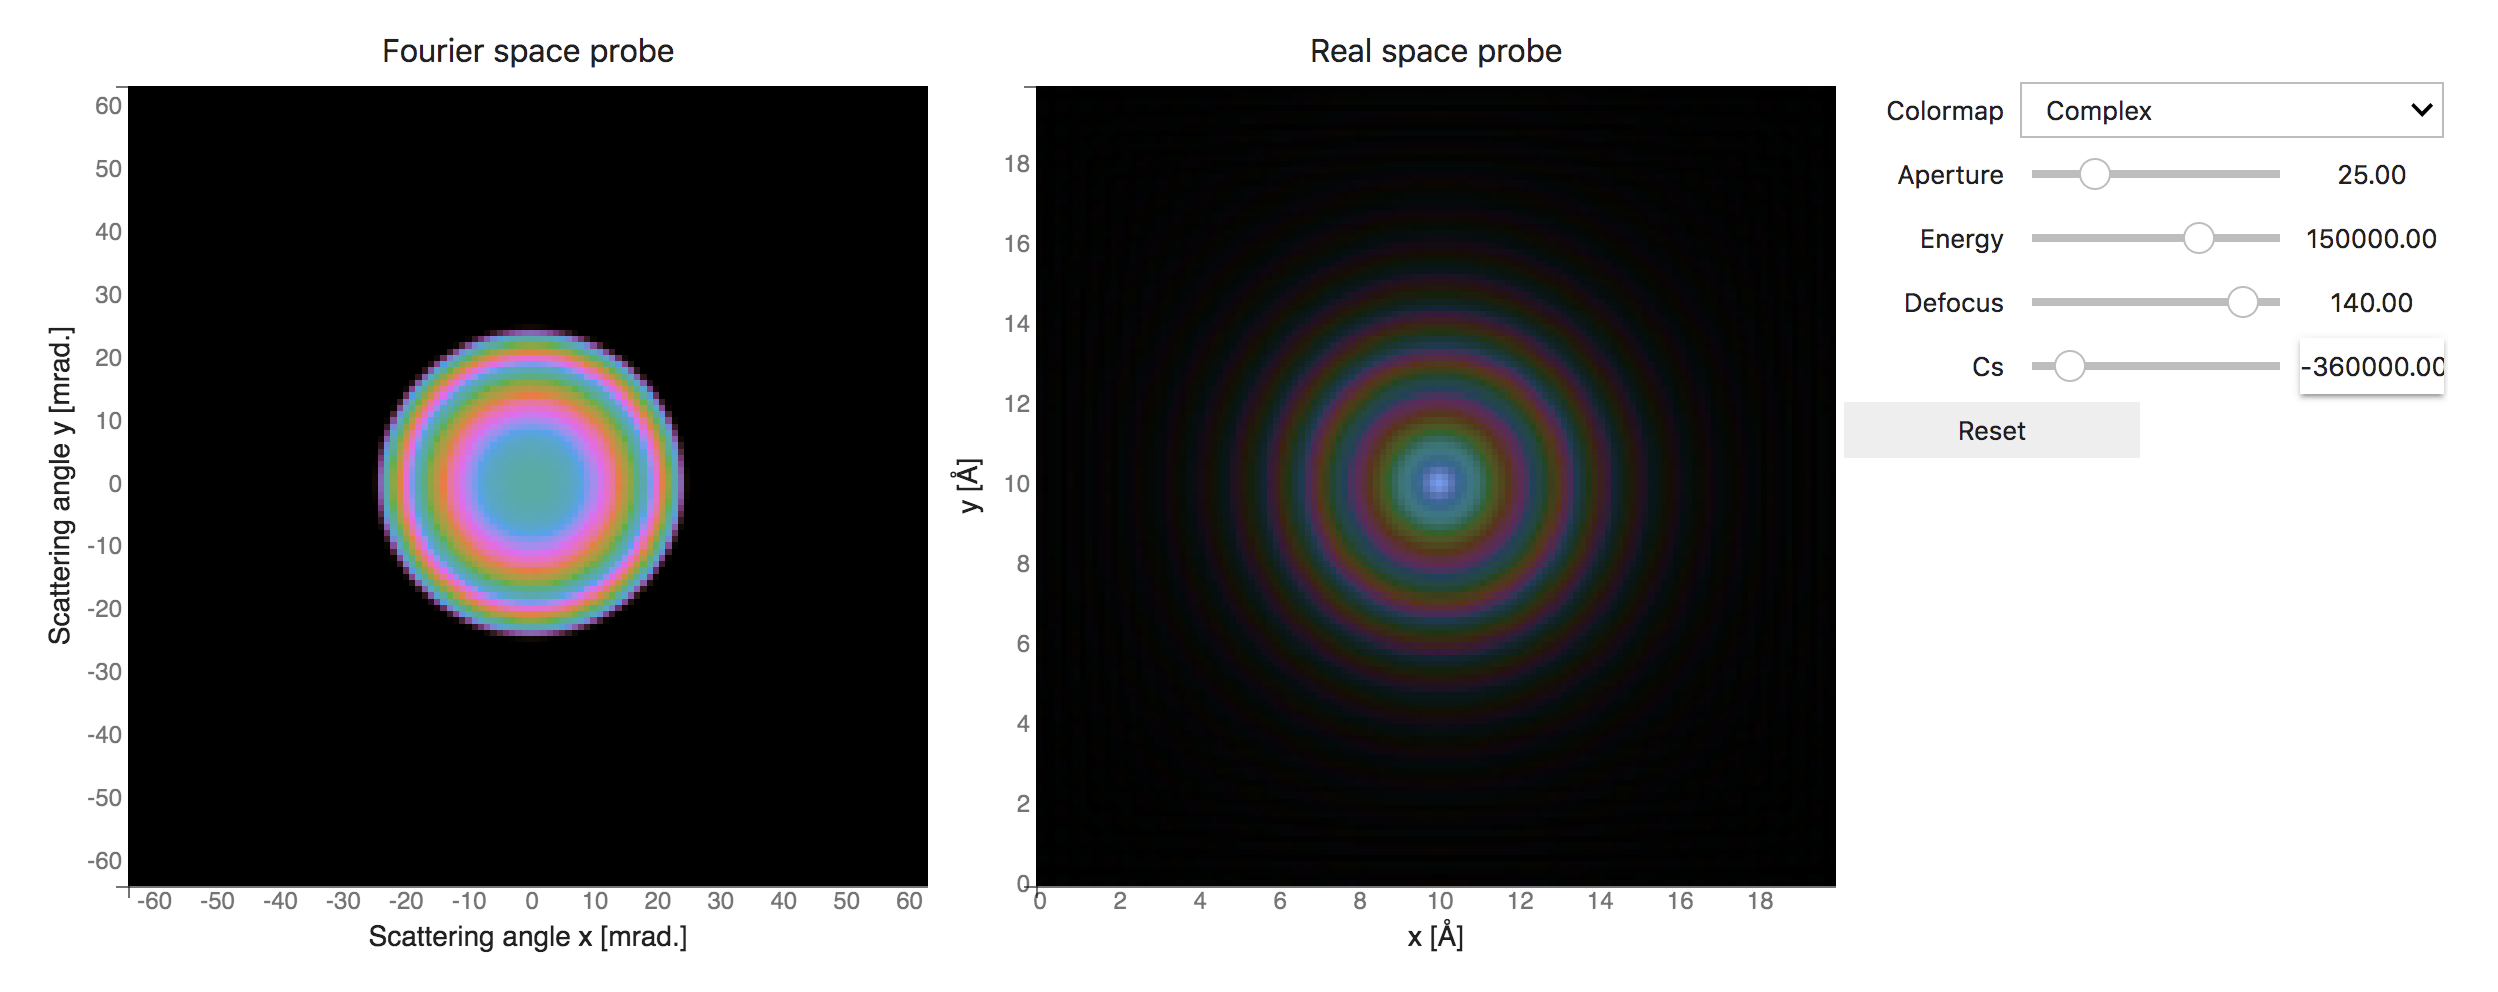
\includegraphics[width=1\textwidth]{figures/probe.png}
    \caption{ \href{https://boiling-wildwood-85903.herokuapp.com/voila/render/probes.ipynb}{(Link to visualization)}
    \textbf{Left} The Fourier space initial wavefunction in Eq. \eqref{eq:fourier_probe}. \textbf{Right} The real space probe at the specimen in Eq. \eqref{eq:realspace_probe}.
    Start by considering the effect of changing just the aperture and energy. In real space, the probe forms the diffraction-limited Airy disk pattern; increasing the aperture or energy decreases the radius of the pattern. Notice that changing the energy shifts the maximum of the axes in Fourier space. This is because the simulation uses a fixed wavefunction sampling; hence the maximum simulated scattering angle is decreased when the energy is increased according to Eq. \ref{}.
    Next, add some defocus. In Fourier space, the phase starts oscillating radially with a linearly decreasing period, the resulting probe grows and its radial intensity profile may have multiple peaks and valleys. Now try to decrease the aperture to include only the inner slowly varying part of the phase; the result is a smaller, more well-behaved probe. Next, add some spherical aberration and try to compensate by adding some defocus to flatten the phase inside the aperture resulting in a better probe.
    Lastly, make a large probe and observe the diffraction fringes from self-interaction. This is the issue that should be avoided by increasing the size of the unit cell, as described in section \ref{}.}
    \label{vis:probe}
\end{figure}




\begin{figure*}[htbp]
    \centering
    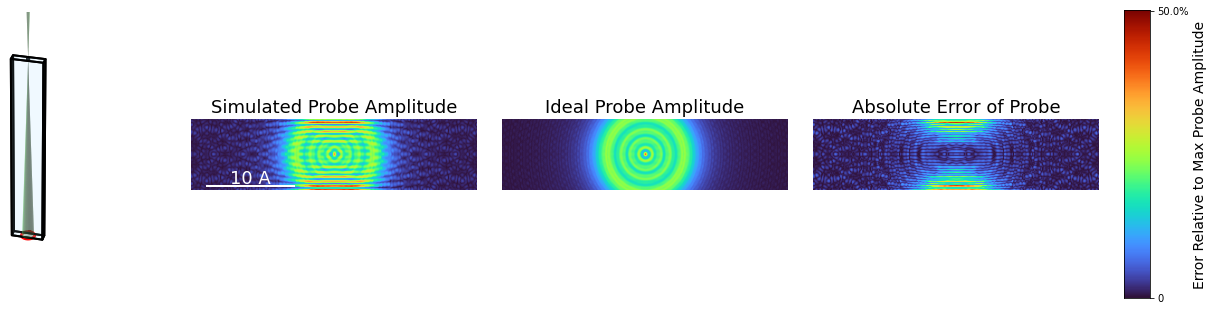
\includegraphics[width=6.4
    in]{figures/probe_overlap.png}
    \caption{{\bf Estimating probe wraparound errors.} - \href{https://github.com/tem-elements/tem-elements/blob/main/notebooks/Probe_overlap.ipynb}{link to notebook}}
    \label{Fig:probe_overlap}
\end{figure*}

Because STEM simulations can require long computation times, we often try to reduce the size of the simulation cell as much as possible. However, we must be careful to use a simulation cell large enough to hold the STEM probe. In particular, we need to consider the size of the probe throughout the full simulation cell volume. For an empty cell, the probe will have a maximum size at either the entrance or exit surface, depending on the probe defocus. 

Fig.~\ref{Fig:probe_overlap} shows an interactive demo for testing the overlap of a STEM probe for different microscope parameters and cell dimensions.  Try setting ...   Note that this example only considers an empty cell volume. Atoms inside the simulation volume will scatter the electron beam, with heavier elements scattering electrons to higher angles. We recommend positioning individual STEM probes at the positions where the highest scattering is expected (for example directly on or adjacent to the thickest atomic columns), and carefully checking the dimensions of the probe at the exit surface. This is especially important for PRISM simulations, as the cropping box around the STEM probe can be significantly smaller than the full cell dimensions for high PRISM interpolation factors \cite{ophus_fast_2017}.







\subsection*{Imaging}
The initial wavefunction is passed through the specimen potential according to the multislice algorithm. The exit wavefunction, $\psi_t(\bm{r}, \bm{r}_p)$, is then diffracted to the detector plane using another Fourier transform
\begin{align*}
    \Psi_t(\bm{k}, \bm{r}_p) = \mathcal{F}_{\bm{r}} [\psi_t(\bm{r}, \bm{r}_p)] .
\end{align*}
The square modulus, $|\Psi_t(\bm{k}, \bm{r}_p)|^2$ is the diffraction pattern for the probe position $\bm{r}_p$. 

Every STEM mode requires calculating a diffraction pattern for each shifted initial wavefunction in the scan region, the modes differ only by how the detector geometry is applied to the diffraction patterns.

In bright-field and annular-dark-field STEM the detector integrates the CBED pattern on a region in the diffraction plane. This is equivalent to multiplying with a detector function
\begin{align*}
    g(\bm{r}_p) = \int\int D(\bm{k}) |\Psi_t(\bm{k}, \bm{r}_p)|^2 \dd^2 \bm{k}
\end{align*}
where 
\begin{align*}
    D(\bm{k}) = 
    \begin{cases}
    1, &  \alpha_a < \lambda k < \alpha_b \\
    0,              & \text{otherwise}
    \end{cases}
\end{align*}
If $D(\bm{k})$ is a small point on the axis then the measurement is a bright field image. If $D(\bm{k})$ is a large annulus covering the high angle scattering then the measurement is an annular dark field image.

The image, $g(\bm{r}_p)$, is the collection of integrated intensities at all sample positions in a (typically) rectangular region. The scan region may be chosen independently of the supercell and may cover only part of the super cell. In the case of a super cell consisting smaller periodic units, computation can be saved by choosing a scan window covering just one of the periodic units.

\begin{figure}[h]
    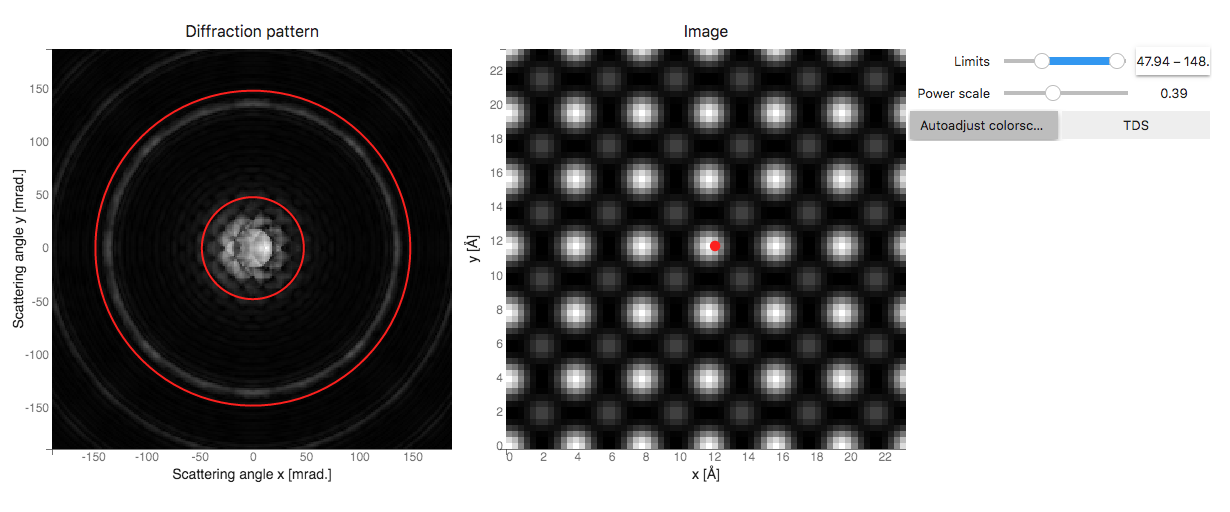
\includegraphics[width=1\textwidth]{figures/annular_integrals.png}
    \caption{ \href{https://boiling-wildwood-85903.herokuapp.com/voila/render/annular_detector.ipynb}{(Link to visualization)}}
    \label{vis:annular}
\end{figure}



% We can significantly limit the computational cost, by choosing the largest possible spacing between the sample positions, or probe step size, $\Delta r_p$. 

% \begin{align*}
%     \Delta r_p = 0.9 \frac{1}{4 \lambda \alpha_{cutoff}}.
% \end{align*}
% It is important to remember the difference between the wavefunction sampling and probe step, both in units of Angstrom. The probe step only refers to the spacing of the initial probe, and it is entirely independent from the grid used to sample the wavefunctions and potentials.

% In Vis. \ref{}, we present a visualization for exploring how the integration region of the detector influence the image.

\subsection*{Differential Phase Contrast}




\subsection*{4D-STEM (CO)}


\section*{Inelastic Scattering}
% Beyond the scope of this article?
% Maybe yeah...

\section*{Including Limited Coherence}





\section*{Post-Processing (HB)}

\subsection*{Limited Electron Dose}

Notebook done, will upload to repository

\subsection*{Elliptical Lens Distortions}

Notebook done, will upload to repository

\begin{figure}[h]
    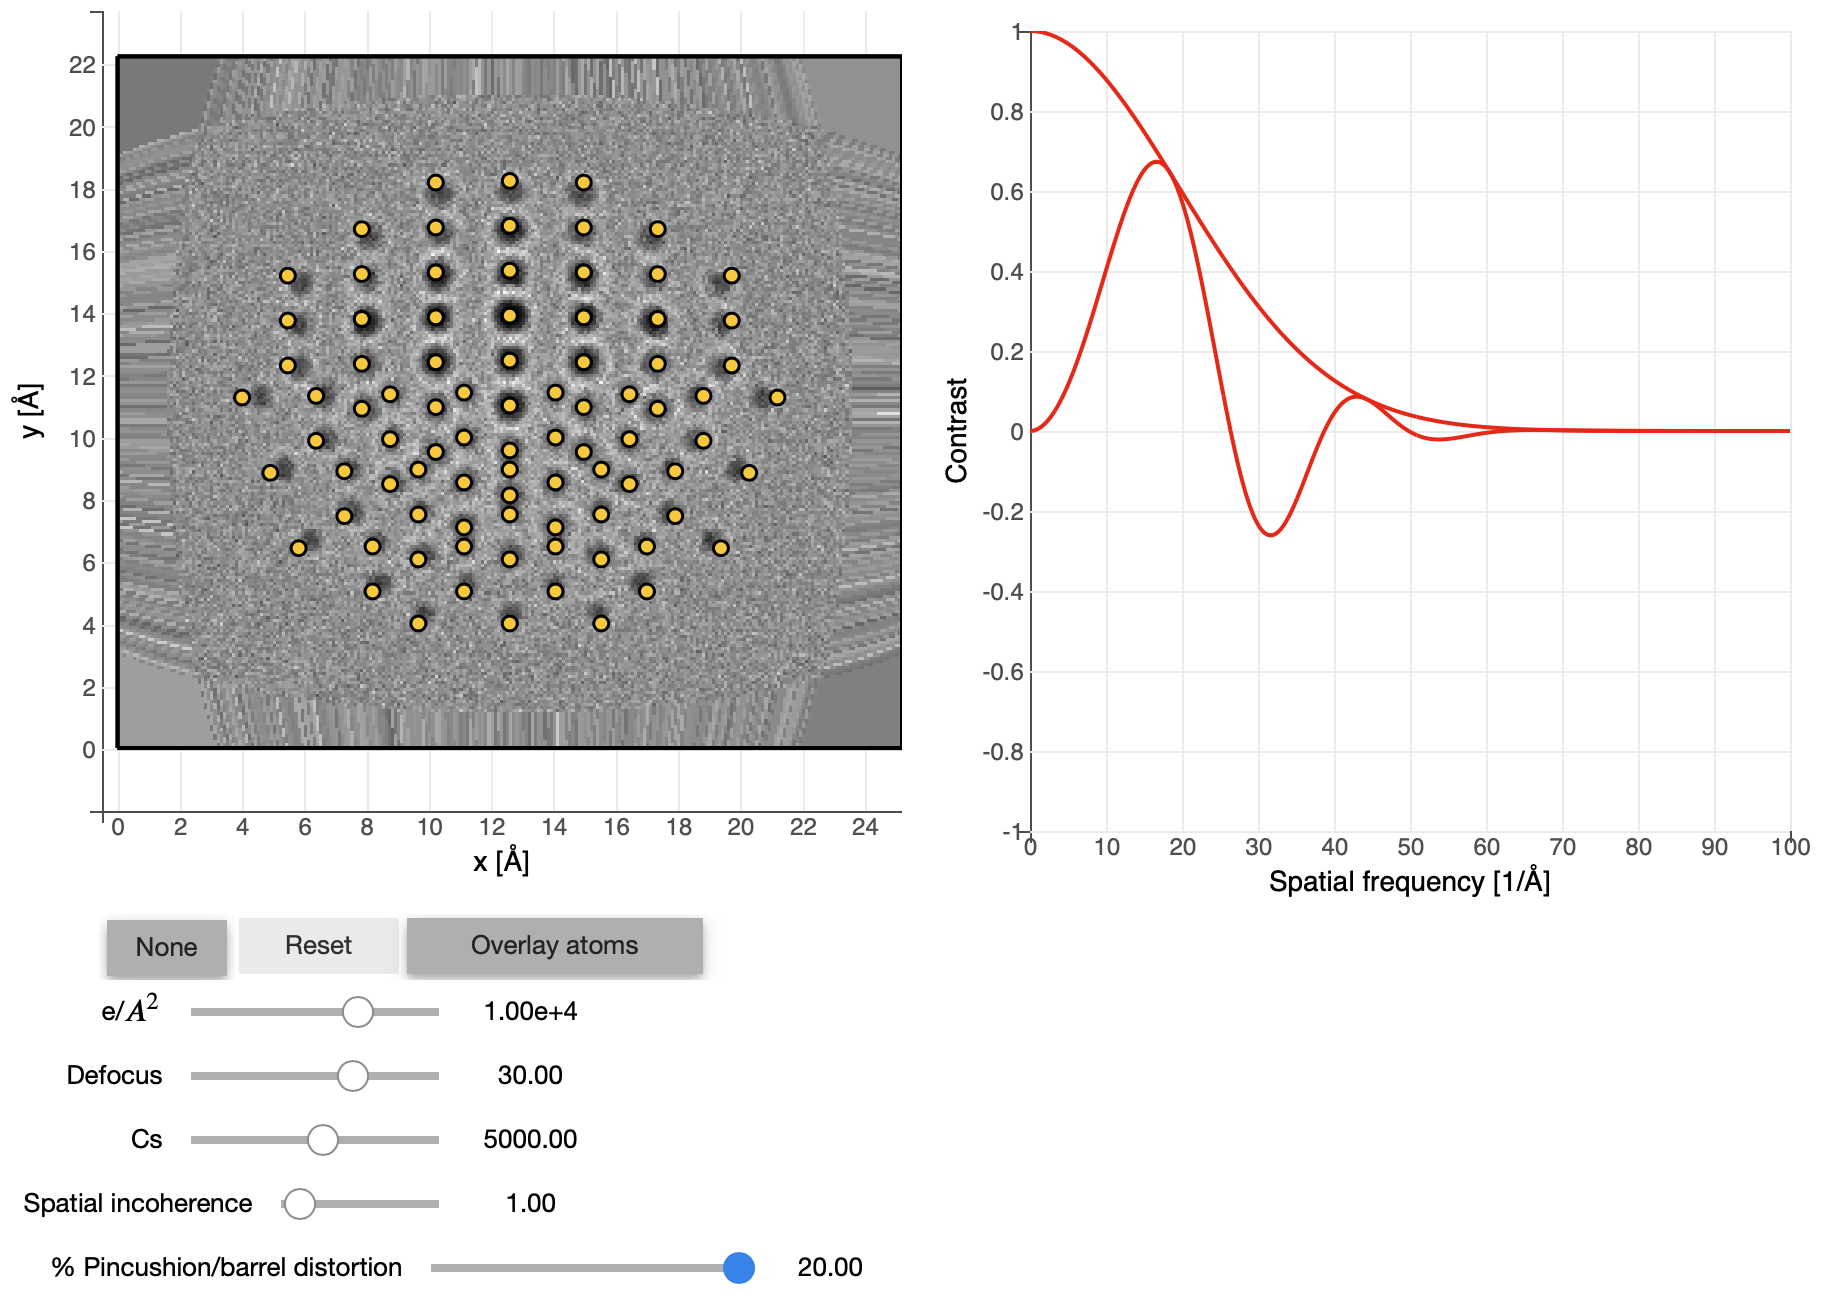
\includegraphics[width=1\textwidth]{figures/dose_distortions.png}
    \caption{ \href{https://tem-elements.herokuapp.com/voila/render/notebooks/dose_distortions.ipynb}{(Link to visualization)}}
    \label{vis:dose_distortions}
\end{figure}

\subsection*{Scanning Artifacts}

probably include



\subsection*{Resampling for Direct Comparison with Experiment}

We can't assume everyone understands nyquist!


\subsection*{Camera MTF and DQE}

Python script written - need to make this interactive (I can help with this AMR)



\section*{Common errors and hints}

Problems:
\begin{itemize}
    \item Sample too thick - make sure the simulation parameters make sense before simulating 
    \item Experiment not plausible, atomic res without sufficient 
    \item Periodic wrapping of probe at the edge of the unit cell
    \item 
\end{itemize}
advice:
\begin{itemize}
    \item for large simulations, run minimal viable simulation to check parameters are good
    \item for large simulations run with multiple frozen phonons, consider running multiple single phonon tasks and adding incoherently. 
    \item for large STEM simulations fields of view, you can split the scan in to into multiple simulations, I think abTEM has a mpipy tutorial for this.   
\end{itemize}



Common errors people do in simulations, or p-hacking simulation, over-fitting, under-determined systems, undersampling



Errors when you don't get it right

How to converge simulations - 

What to do when you don't know a microscope parameter

When to use an ab initio potential and when it is not necessary


\section*{Possible other sections to include}



\section*{Conclusion and Outlook}


Conclusion 
Datasets are getting more complex and simulations can aid in interpreting the information 
Can simulate experiment to inform optimal experimental parameters, feasibility 
Can 

Outlook 
ML 
In-situ 


\section*{Acknowledgements}

We are heavily indebted to the various excellent textbooks on electron microscopy, in particular \cite{kirkland2020}, add others ...   


%\section*{References}
% \bibliographystyle{MandM}
\bibliography{refs,toma_references}


\appendix 
\section{Numerical values of constants}\label{app:constants}

The values of commonly used constants in SI units are
\begin{center}
\begin{tabular}{l l l} 
    \hline
    constant & value & units \\
    \hline
    $h$ & $6.62607 \cdot 10^{-34}$ & m$^2$kg/s   \\
    $c$ & $2.99792458 \cdot 10^{8}$ & m/s  \\ 
    $e$ & $1.602177 \cdot 10^{-19}$ & C (A$\,$s)  \\ 
    $m$ & $9.109383 \cdot 10^{-31}$ & kg  \\ 
    \hline
\end{tabular}
\end{center}

\end{document}